\documentclass{../template/note}

\author{Oliver West}
\title{Differential Equations}
\date{}

\begin{document}

    \maketitle

    \tableofcontents

    \lecture{Lecture 1 -- 10/10/25}

    \setcounter{section}{-1}
    \section{Introduction}

    Differential equations appear in almost all branches of science and applied mathematics.

    \begin{example}
        Newton's second law:
        \begin{align*}
            m \frac{d^2x}{dt^2} = F(x,t)
        \end{align*}
        where \(m\) is mass, \(F\) is force -- relates rate of change of position \(x\), the \emph{dependent variable}, with time \(t\), the \emph{independent variable}. 
    \end{example}

    \noindent How do we solve such equations?

    \section{Calculus}

    \subsection{Basic calculus}

    \subsubsection{Differentiation}
    
    \begin{definition}
        The derivative of a function \(f(x)\) with respect to its argument \(x\) is the function
        \begin{align*}
            \frac{df}{dx}=\lim_{h\to 0}\frac{f(x+h)-f(x)}{h}
        \end{align*}

        \begin{figure}[ht]
            \centering
            \incfig{0.4\textwidth}{derivative-diagram}
            \caption{The derivative at \(x\) is the slope of the red line as \(h\) approaches 0.}
            \label{fig:derivative-diagram}
        \end{figure}
    
    \end{definition}

    \begin{remark*}[Limits]
        Informally, if \(\lim_{x\to x_0}f(x) = A\), then \(f(x)\) can be made arbitrarily close to \(A\) by making \(x\) sufficiently close to \(x_0\) (not necessary for \(f(x_0) = A\) itself). See notes/Analysis I for a more formal discussion.
    \end{remark*}
    
    
    For the derivative to exist, we require that the left handed limit (\(\lim_{h\to 0^-}\)) and the right handed limit (\(\lim_{h\to 0^+}\)) both exist and are equal.

    \begin{example}
        \(|x|\) is not differentiable at \(x=0\) (positive limit \(1\), negative limit \(-1\)).
    \end{example}

    Also note other common notations for the derivative: \(f'(x), \dot f(x)\). The second one is normally used when differentiating with respect to time.

    For sufficiently smooth functions, we can also define higher derivatives. Notation is as follows:
    \begin{align*}
        \frac{d}{dx} \left(\frac{df}{dx}\right) = \frac{d^2f}{dx^2} &= f''(x) = \ddot f(x) \\
        \frac{d^nf}{dx^n} &= f^{(n)}(x)
    \end{align*}

    \subsubsection{Order parameters}

    Want to compare the behaviour of functions close to a limiting point \(x_0\).

    \begin{definition}[Big O notation]
        Loosely, big O means `can be bounded by'.
        \begin{enumerate}[label=Case \arabic*.,leftmargin=55px]
            \item \(x_0\) finite, then \(f(x)\) is \(O(g(x))\) as \(x \to x_0\) if there exist \(\delta > 0\) and \(M > 0\) such that, for any \(x\) with \(0 < |x-x_0| < \delta\), \(|f(x)| \leq M|g(x)|\).
            \item \(x_0 = \infty\), then \(f(x)\) is \(O(g(x))\) as \(x \to \infty\) if there exist \(x_1\) and \(M > 0\) such that, for any \(x > x_1\), \(|f(x)| \leq M|g(x)\).
        \end{enumerate}
        We often write \(f(x) = O(g(x))\), but this equals sign is an abuse of notation.
    \end{definition}

    \begin{remark*}
        If \(f(x) = O(g(x))\), it follows that \(\frac{f(x)}{g(x)}\) is bounded as \(x \to x_0\).
    \end{remark*}

    
    Here are some examples with \(x_0 = 0\).
    
    \begin{figure}[ht]
        \centering
        \incfig{0.4\textwidth}{big-O-demo}
        \caption{\(x \neq O(x^2)\) as \(x \to 0\) \\ \(x^2 = O(x)\) as \(x \to 0\) \\ \(x = O(\sqrt x)\) as \(x \to 0\)}
        \label{fig:big-O-demo}
    \end{figure}
    
    Another example: \(\sin 2x = O(x)\) since \(|\sin 2x| \leq 2|x|\).
    
    Example with \(x_0 = \infty\), then \(2x^3 + 4x = O(x^3)\) as \(x \to \infty\) -- for any \(x > 1\), \(|2x^3 + 4x| \leq 2|x^3| + 4|x| \leq 6|x^3|\).

    \begin{definition}[Little o]
        Loosely, little o means `much smaller than'. Sometimes in handwriting it is written \(\underline o\) to distinguish from big O.

        \(f(x)\) is \(o(g(x))\) as \(x \to x_0\) if, for any \(\varepsilon > 0\), there exists \(\delta > 0\) such that, for all \(x\) with \(0 < |x-x_0| < \delta\), \(|f(x)| \leq \varepsilon|g(x)|\).

        \emph{Key difference}: we can pick our \(\varepsilon\) arbitrarily large, unlike with big O.

        If \(g \neq 0\) in the vicinity of \(x_0\) (but not necessarily at \(x_0\)), then, equivalently,
        \begin{align*}
            \lim_{x\to x_0} \frac{f(x)}{g(x)} = 0
        \end{align*}

        We make the same abuse of notation, writing \(f(x) = o(g(x))\). We have a separate case for \(x_0\) infinite which is analogous to big O.
    \end{definition}

    \begin{example}
        \(x^2 = o(x)\) as \(x \to 0\), since
        \begin{align*}
            \lim_{x \to 0}\frac{x^2}{x} = \lim_{x \to 0} x = 0
        \end{align*}
        
        \(\sqrt x = o(x)\) \emph{as \(x \to \infty\)}, since
        \begin{align*}
            \lim_{x \to \infty}\frac{\sqrt x}{x} = \lim_{x \to \infty} \frac{1}{\sqrt x} = 0
        \end{align*}
        
        
    \end{example}

    \begin{remark*} Note
        \begin{itemize}
            \item \(f(x) = o(g(x))\) is a stronger statement than \(f(x) = O(g(x))\) -- in particular, \(f(x) = o(g(x)) \implies f(x) = O(g(x))\). \emph{Remember: \(o\) is bounded by any multiple, \(O\) is bounded by some multiple}. For example, \(2x = O(x)\), but \(2x \neq o(x)\).
            \item Constants don't matter. If \(f(x) = O(g(x))\) then \(af(x) = O(g(x))\) and \(f(x) = O(ag(x))\).
        \end{itemize}
    \end{remark*}
    
    \noindent Order parameters are often useful for classifying remainder terms before taking limits. For example, for some finite \(h\),
    \begin{align*}
        f(x_0+h) - f(x_0) &= hf'(x_0) + \varepsilon(h) \\
        \implies \lim_{h \to 0}\frac{f(x_0+h)-f(x)}{h} &= f'(x_0) + \lim_{h \to 0} \frac{\varepsilon(h)}{h}
    \end{align*}

    where \(\varepsilon(h)\) is just some remainder term depending on \(h\). For the derivative to exist, this \(\frac{\varepsilon(h)}{h}\) vanishes, so we conclude \(\varepsilon(h) = o(h)\) as \(h \to 0\). Thus

    \begin{align*}
        f(x_0 + h) = f(x_0) + hf'(x_0) + o(h)
    \end{align*}
    
    as \(h \to 0\).

    \lecture{Lecture 2 -- 13/10/25}

    \subsubsection{Rules for differentiation}

    \begin{theorem}[Chain rule]
        Let \(f(x) = F(g(x))\), then
        \begin{align*}
            \frac{df}{dx} = F'(g(x))\frac{df}{dx} = \frac{dF}{dg}\cdot\frac{dg}{dx}
        \end{align*}
        
        
    \end{theorem}

    \begin{example}
        \[
            \frac{d}{dx}\left(\sin(x^2-x+2)\right) = \cos(x^2-x+2) \cdot (2x-1)
        \]
        
        
    \end{example}
    
    \begin{theorem}[Product rule]
        Given \(f(x) = u(x)v(x)\),
        \[
            \frac{df}{dx} = v \frac{du}{dx} + u \frac{dv}{dx}
        \]
        Proof on example sheet 1.
    \end{theorem}
    
    \begin{theorem}[Quotient rule]
        Really a special case of the product rule where instead of \(v\) we have \(1/v\).
        \[
            \frac{d}{dx} \left(\frac{u}{v}\right) = \frac{vu'-uv'}{v^2}
        \]
    \end{theorem}
    
    \begin{theorem}[Leibniz's rule/generalised product rule]
        Let \(f(x) = u(x)v(x)\), then
        \[
            f^{(n)}(x) = \sum_{r=0}^n \binom{n}{r} u^{(n-r)}(x) v^{(r)}(x) 
        \]
    \end{theorem}
    
    \subsubsection{Taylor series}

    Might want to approximate the behaviour of a function in a small neighbourhood, and also quantify exactly how good it is.


    \begin{definition}
        For \(f(x)\) infinitely differentiable at \(x=x_0\), the \emph{Taylor series} around \(x_0\) is given by
        \begin{align*}
            T_f(x) &= f(x_0) + (x-x_0)f'(x_0) + \frac{1}{2!}(x-x_0)^2f''(x_0) + \dots \\
            &= \sum_{r=0}^\infty \frac{1}{r!}(x-x_0)^rf^{(r)}(x_0)
        \end{align*}
    \end{definition}
    
    \begin{definition}
        The \emph{Taylor polynomial} of degree \(n\), \(P_n(x)\), is obtained by truncating the Taylor series after the term of degree \(n\) -- that is,
        \begin{align*}
            P_n(x) &= f(x_0) + (x-x_0)f'(x_0) + \dots + \frac{1}{n!}(x-x_0)^n f^{(n)}(x_0) \\
            &= \sum_{r=0}^n \frac{1}{r!}(x-x_0)^rf^{(r)}(x_0)
        \end{align*}
        Intuition: this matches the first \(n\) derivatives of \(f\).
        
    \end{definition}
    
    How good of an approximation is a Taylor polynomial?

    Recall \(f(x_0+h)=f(x_0)+hf'(x_0)+o(h)\) as \(h \to 0\). So the Taylor polynomial of degree 1 has error \(o(h)\). We can extend this result to Taylor's theorem.

    \begin{theorem}[Taylor's theorem]
        For an \(n\)-times differentiable function \(f(x)\) at \(x_0\),
        \begin{align*}
            f(x_0+h) = f(x_0) + hf'(x_0) + \frac{1}{2!}h^2f''(x_0) + \dots + \frac{1}{n!}h^n f^{(n)}(x_0) + E_n
        \end{align*}
        where \(E_n = o(h^n)\) as \(h \to 0\). \\
    
        We have a stronger version if \(f\) is \(n+1\)-times differentiable in the open interval \((x_0, x_0+h)\), and \(f^{(n+1)}(x)\) is continuous in this interval. Then
        \begin{align*}
            E_n &= \frac{1}{(n+1)!}h^{n+1}f^{(n+1)}(x_n)
        \end{align*}
        
        for some \(x_n\) with \(x_0 \leq x_n \leq x_0+h\), and from this it clearly follows that \(E_n = O(h^{n+1})\) as \(h \to 0\).
        
        
    \end{theorem}
    
    \begin{remark*}
        Note that \(O(h^{n+1})\) is stronger than \(o(n)\). For example, \(h^{n+\frac 1 2}\) is \(o(h^n)\) but not \(O(h^{n+1})\) as \(h \to 0\).
    \end{remark*}
    
    When \(x = x_0 + h\), then Taylor's theorem becomes \(f(x) = P_n(x) + E_n\). So \(P_n(x)\) does indeed provide a local approximation to \(f(x)\) in the vicinity of \(x_0\) with error \(o(h^n)\) or \(O(h^{n+1})\).

    Furthermore, if \(\lim_{n \to \infty}E_n = 0\), then the full Taylor series converges to \(f(x)\).
    
    \begin{example}
        Take \(f(x) = \exp(x)\) around \(x_0 = 0\). We can use the stronger form:
        \begin{align*}
            E_n = \frac{1}{(n+1)!}h^{n+1}\exp(x_n)
        \end{align*}
        where \(0 \leq x_n \leq h\) (we assume \(h > 0\).) Consider the fractional error:
        \begin{align*}
            \frac{E_n}{\exp(h)} &= \frac{1}{(n+1)!}h^{n+1}\exp(x_n-h) \\
            &\leq \frac{h^{n+1}}{(n+1)!}
        \end{align*}
        
        \noindent So if we have a particular `target accuracy', this tells us how large our \(n\) has to be.
        
    \end{example}
    
    \subsubsection{L'H\^opital's rule}

    Allows us to deal with limits of indeterminate forms.

    \begin{theorem}[L'H\^opital's rule]
        Let \(f(x)\) and \(g(x)\) be differentiable at \(x=x_0\) with continuous first derivatives there, and suppose
        \begin{align*}
            \lim_{x \to x_0}f(x) = f(x_0) &= 0 \\
            \lim_{x \to x_0}g(x) = g(x_0) &= 0
        \end{align*}
        Then, if \(g'(x) \neq 0\) in the vicinity of \(x_0\),

        \[
            \lim_{x \to x_0} \frac{f(x)}{g(x)} = \lim_{x \to x_0} \frac{f'(x)}{g'(x)}
        \]
        provided this limit exists.
        
    \end{theorem}
    
    \begin{proof}
        By Taylor's theorem, \(f(x) = f(x_0) + (x-x_0)f'(x_0) + o(x-x_0)\), and \(g(x) = g(x_0) + (x-x_0)g'(x_0) + o(x-x_0)\) as \(x \to x_0\). But \(f(x_0) = g(x_0) = 0\), so

        \begin{align*}
            \lim_{x \to x_0} \frac{f(x)}{g(x)} &= \lim_{x\to x_0}\frac{(x-x_0)f'(x_0) + o(x-x_0)}{(x-x_0)g'(x_0) + o(x-x_0)} \\
            &= \lim_{x\to x_0}\frac{f'(x_0) + \frac{o(x-x_0)}{x-x_0}}{g'(x_0) + \frac{o(x-x_0)}{x-x_0}} \\
            &= \frac{\lim_{x\to x_0}\left(f'(x_0) + \frac{o(x-x_0)}{x-x_0}\right)}{\lim_{x\to x_0}\left(g'(x_0) + \frac{o(x-x_0)}{x-x_0}\right)} \\
            &= \frac{f'(x_0)}{g'(x_0)} \\
            &= \lim_{x \to x_0} \frac{f'(x)}{g'(x)}
        \end{align*}
        
        where the final line is by continuity of the first derivative.
        
    \end{proof}

    \begin{remark*}
        This also works if \(f\), \(g\) both go to infinity instead of 0.
    \end{remark*}

    \lecture{Lecture 3 -- 15/10/25}

    L'H\^opital's rule can be generalised -- just keep taking derivatives until we eventually don't have an indeterminate form anymore.

    \begin{example}
        \begin{align*}
            f(x) &= 3 \sin x - \sin 3x \\
            g(x) &= 2x - \sin 2x
        \end{align*}
        We must go to the third derivative to evaluate \(\lim_{x \to 0}\frac{f(x)}{g(x)}\).        
    \end{example}
    
    \subsection{Integration}

    Two notions of integration:

    \begin{itemize}
        \item the area under a curve (Riemann sum);
        \item the inverse of differentiation.
    \end{itemize}
    
    \subsubsection{Integrals as Riemann sums}

    \begin{definition}
        The \emph{integral} of a suitably well-defined function \(f(x)\) is the limit of a sum of the form:
        \[
            \int_a^b f(x) dx = \lim_{N \to \infty} \sum_{n=0}^{N-1} f(x_n)\Delta x 
        \]
        where \(\Delta x = \frac{b-a} n\) and \(x_n = a + n\Delta x\).

        \begin{figure}[ht]
            \centering
            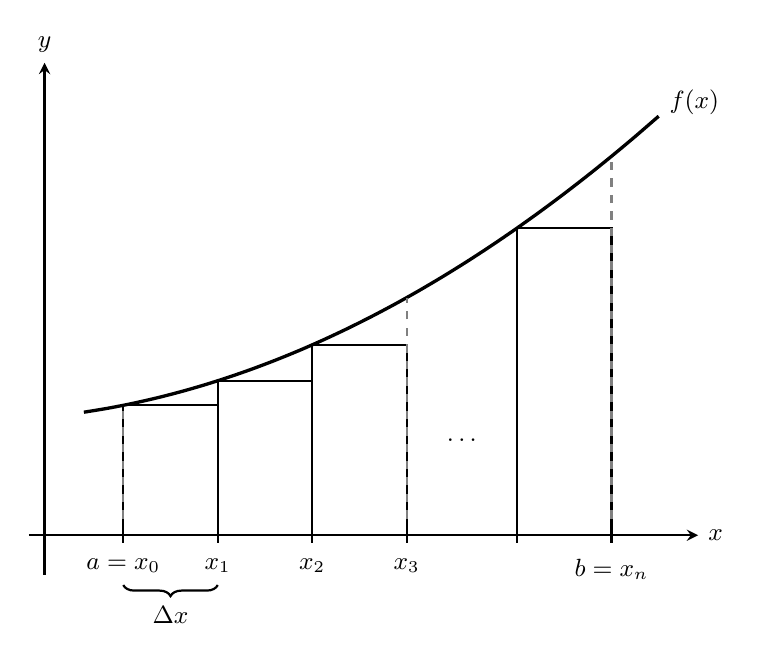
\begin{tikzpicture}[
                thick,          % Set line thickness
                >=stealth,      % Set arrow tip style
                font=\small     % Use a slightly smaller font for labels
            ]

            % 1. Define a convex, always-increasing function (and lower)
            \tikzset{declare function={myfunc(\x)=0.05*\x*\x + 0.1*\x + 1.5;}} 
            % Vertex is at x=-1, so it's increasing for all x > -1

            % 2. Define the partitions (a != 0, increased gap)
            \def\a{1.0}      % a = x_0, now starts at 1.0
            \def\dx{1.2}     % Delta x, consistent spacing
            \def\xone{\a + \dx}
            \def\xtwo{\a + 2*\dx}
            \def\xthree{\a + 3*\dx}
            \def\xnminusone{6.0} % Still arbitrary for visual spacing
            \def\b{7.2}      % b = x_n

            % Adjust x-axis start to account for new 'a'
            \def\xminaxis{-0.2}
            \def\xmaxaxis{7.8}

            % 3. Draw the rectangles (Left Riemann Sum), not blue
            \draw[draw=black] % Only draw outline, no fill
                (\a, 0) rectangle (\xone, {myfunc(\a)});
            \draw[draw=black] 
                (\xone, 0) rectangle (\xtwo, {myfunc(\xone)});
            \draw[draw=black] 
                (\xtwo, 0) rectangle (\xthree, {myfunc(\xtwo)});
            % The final rectangle
            \draw[draw=black] 
                (\xnminusone, 0) rectangle (\b, {myfunc(\xnminusone)});

            % 4. Draw the smooth function graph
            \draw[domain=\a-0.5:\xmaxaxis, smooth, variable=\x, black, very thick] 
                plot ({\x}, {myfunc(\x)}) node[right, yshift=5pt] {\(f(x)\)}; % f(x) label

            % 5. Draw the axes
            \draw[->] (\xminaxis, 0) -- (\xmaxaxis+0.5, 0) node[right] {\(x\)};
            % Adjust y-axis height for new function
            \draw[->] (0, -0.5) -- (0, 6) node[above] {\(y\)}; % y-axis label

            % 6. Add labels and ticks on the x-axis
            % Boundary lines at a and b
            \draw[dashed, gray] (\a, 0) -- (\a, {myfunc(\a)});
            \draw (\a, 0.1) -- (\a, -0.1) node[below=2pt] {\(a=x_0\)}; % Added tick
            
            \draw[dashed, gray] (\b, 0) -- (\b, {myfunc(\b)});
            \draw (\b, 0.1) -- (\b, -0.1) node[below=2pt] {\(b=x_n\)}; % Added tick
            
            % Ticks for intermediate points
            \draw (\xone, 0.1) -- (\xone, -0.1) node[below=2pt] {\(x_1\)};
            \draw (\xtwo, 0.1) -- (\xtwo, -0.1) node[below=2pt] {\(x_2\)};
            
            % --- NEW LINE ADDED HERE ---
            \draw[dashed, gray] (\xthree, 0) -- (\xthree, {myfunc(\xthree)}); 
            \draw (\xthree, 0.1) -- (\xthree, -0.1) node[below=2pt] {\(x_3\)};
            
            \draw (\xnminusone, 0.1) -- (\xnminusone, -0.1); % Unlabelled tick

            % Ellipsis - moved up
            \node at ( {(\xthree + \xnminusone) / 2} , {myfunc(\xtwo) / 2} ) {\(\dots\)};

            % 7. Add the Delta x label
            \draw [
                decorate,
                decoration={brace, amplitude=4pt, mirror},
                yshift=-18pt % Kept low to avoid overlap
                ] (\a, 0) -- (\xone, 0) 
                node [midway, below=4pt] {\(\Delta x\)};

            \end{tikzpicture}
            \caption{Graphical representation of a Riemann sum}
            \label{fig:riemann-sum}
        \end{figure}

        \(f(x)\) is \emph{Riemann integrable} over this range if the value of the sum doesn't depend on the choice of rectangles in the limit as \(\Delta x \to 0\) (for example, we're allowed to have some \(\Delta x\)'s bigger than others).
        
        
    \end{definition}

    \begin{figure}[ht]
        \centering
        \incfig{0.4\textwidth}{riemann-sum-proof}
        \caption{Riemann sum zoomed in on one rectangle}
        \label{fig:riemann-sum-proof}
    \end{figure}
    
    

    By the \emph{mean value theorem}, for \(f(x)\) continuous, the area under the curve from \(x_n\) to \(x_{n+1}\) is
    \begin{align*}
        A_n &= (x_{n+1}-x_n)f(c_n) \\
        &= \Delta x f(c_n)
    \end{align*}
    
    for some \(c_n\), \(x_n \leq c_n \leq x_{n+1}\). Furthermore, if \(f(x)\) differentiable, Taylor's theorem gives

    \begin{align*}
        f(c_n) &= f(x_n) + O(c_n-x_n) && \text{as } c_n - x_n \to 0 \\
        &= f(x_n) + O(\Delta x) && \text{since } \Delta x \geq c_n - x_n
    \end{align*}
    
    Hence
    \[
        A_n = \Delta x f(x_n) + O[(\Delta x)^2]
    \]
    as \(\Delta x \to 0\).
    
    Then
    \begin{align*}
        A &= \lim_{N \to \infty} \sum_{n=0}^{N-1} A_n \\
        &= \lim_{N \to \infty} \sum_{n=0}^{N-1} f(x_n) \Delta x + \lim_{N \to \infty} N \cdot O[(\Delta x)]^2 \\
        &= \lim_{N \to \infty} \sum_{n=0}^{N-1} f(x_n) \Delta x + \lim_{N \to \infty}  \underbrace{N \cdot O\left[\left(\frac{b-a}{N}\right)^2\right]}_{O(1/N)} \\
        &= \int_a^b f(x) dx + 0
    \end{align*}
    
    \subsubsection{Fundamental theorem of calculus (FTC)}
    
    \begin{theorem}[FTC]
        Let
        \[
            F(x) = \int_a^x f(t) dt
        \]
        then
        \[
            \frac{dF}{dx} = \frac{d}{dx} \left[\int_a^x f(t) dt\right] = f(x)
        \]
    \end{theorem}

    \begin{proof}
        \begin{align*}
            \frac{dF}{dx} &= \lim_{h \to 0} \frac {F(x+h)-F(x)} h \\
            &= \lim_{h \to 0} \frac 1 h \left[\int_a^{x+h} f(t) dt-\int_a^x f(t) dt\right] \\
            &= \lim_{h \to 0} \frac 1 h \left[\int_x^{x+h} f(t) dt\right] \\
            &= \lim_{h \to 0} \frac 1 h \left[f(x)h + O(h^2)\right] && \text{by MVT + Taylor} \\
            &= \lim_{h \to 0} f(x) + O(h) \\
            &= f(x)
        \end{align*}
    \end{proof}
    
    \begin{remark*}
        \(F(x)\) is a solution to the differential equation \(\frac{dF}{dx} = f(x)\) with \(F(a) = 0\).
    \end{remark*}

    \begin{corollary}
        If we're differentiating w.r.t the other limit, we have
        \[
            \frac{d}{dx} \int_x^b f(t) dt = -f(x)
        \]
        Furthermore, 
        \begin{align*}
            \frac{d}{dx} \int_a^g(x) f(t) dt &= \frac{d}{dx} F(g(x)) \\
            &= \frac{dF}{dg} \cdot \frac{dg}{dx} \\
            &= f(g(x)) \frac{dg}{dx}
        \end{align*}
        and we could also do this with the lower limit instead.
    \end{corollary}
    
    \begin{definition}
        The \emph{indefinite integral} \(\int f(x) dx\) or \(\int^x f(t) dt\) is the same as the definite integral from a constant to \(x\), except that it has an integration constant given by the unspecified lower limit.
    \end{definition}
    
    \subsubsection{Integration techniques}

    \begin{itemize}
        \item \emph{Substitution}. If the integrand contains a function of a function, it might help to substitute the inner function.
        
        For example, consider \(I = \int \frac{1-2x}{\sqrt{x-x^2}} dx\). Let \(u=x-x^2\), then \(\frac{du}{dx} = 1-2x\), so
        \begin{align*}
            I &= \int \frac{1}{\sqrt u}\; du \\
            &= 2\sqrt u + c \\
            &= 2\sqrt{x-x^2} + c
        \end{align*}

        \item \emph{Trigonometric substitutions}. Recall some important identities:
        \begin{align*}
            \cos^2 \theta + \sin^2 \theta &= 1 \\
            1 + \tan^2 \theta &= \sec^2 \theta 
        \end{align*}
        \begin{align*}
            \cosh^2 u - \sinh^2 u &= 1 \\
            1 - \tanh^2 u &= \sech^2 u
        \end{align*}

        Using these identities, we can make up some `recommended' substitutions for expressions that might appear in the integral.

        \begin{center}
        
            \begin{tabular}{r l}
                \(\sqrt{1-x^2}\) & \(x = \sin \theta\) \\
                \(1 + x^2\) & \(x = \tan \theta\) \\
                \(\sqrt{x^2 + 1}\) & \(x = \sinh u\) \\
                \(\sqrt{x^2 - 1}\) & \(x = \cosh u\) \\
                \(1-x^2\) & \(x = \tanh u\) \\
            \end{tabular}
            
        \end{center}
        
        For example, consider
        \begin{align*}
            I &= \int \sqrt{2x - x^2} \; dx \\
            &= \int \sqrt{1 - (x-1)^2} \; dx
        \end{align*}
        Put \(x-1 = \sin \theta \implies dx = \cos \theta d\theta\) -- if we want to worry about uniqueness, just say \(x\) is between 0 and 2. Then
        \begin{align*}
            I &= \int \sqrt{\cos^2 \theta} \cos \theta \; d \theta \\
            &= \int \cos^2 \theta \; d \theta \\
            &= \frac{1}{2} \int 1 + \cos 2 \theta d \theta \\
            &= \frac{1}{2} (\theta + \frac 1 2 \sin 2 \theta) + c \\
            &= \frac{1}{2} (\theta + \sin \theta \cos \theta) + c \\
            &= \frac{1}{2} \left(\arcsin(x-1) + (x-1)\sqrt{1-(x-1)^2}\right) + c
        \end{align*}
        
    \end{itemize}
    
    \lecture{Lecture 4 -- 17/10/25}

    \begin{itemize}[resume]
        \item \emph{Integration by parts}. Recall
        \begin{align*}
            (uv)' &= u'v + v'u \\
            \implies \int uv'\; dx &= uv - \int u'v\; dx
        \end{align*}
        by integrating on both sides and rearranging.

        \begin{enumerate}[label=\protect\circled{\arabic*}]
            \item Consider \(\int_0^\infty xe^{-x} \; dx\) -- choose \(u = x\), \(v' = e^{-x}\), so \(u' = 1\), \(v = -e^{-x}\). Hence
            \begin{align*}
                \int_0^\infty xe^{-x} \; dx &= \left[-xe^{-x}\right]_0^\infty - \int_0^\infty -e^{-x} \; dx \\
                &= 0 + [-e^{-x}]_0^\infty \\
                &= 1
            \end{align*}
            \item Consider \(\int \ln x \; dx\) -- choose \(u = \ln x\), \(v' = 1\), so \(u' = 1/x\), \(v = x\). Thus
            \begin{align*}
                \int \ln x \; dx &= x \ln x - \int \frac{1}{x} \cdot x \; dx \\
                &= x \ln x - x + c
            \end{align*}
            This \(v' = 1\) method also works for inverse trig and hyperbolic trig functions.
            
            
        \end{enumerate}
        
        
        
    \end{itemize}
    
    \subsection{Partial differentiation}

    \subsubsection{Functions of several variables}

    We want to generalise the notion of differentiation to functions of more than one variable -- \emph{multivariate functions}.

    \begin{example}
        Lots of things depend on two variables!
        \begin{itemize}
            \item Height of terrain, \(h(x,y)\);
            \item Temperature in a room, \(T(x, y, z, t)\);
            \item Pressure of a gas as a function of volume and temperature, \(P(V, T)\).
        \end{itemize}
        
        
    \end{example}
    
    How can we represent these multivariate functions? We can use a \emph{contour plot}, as on a topographic map.

    DIAGRAM: on x-y axes, positive only some circularish lines, labelled \(f(x, y)\) = const. Red point labelled A.

    We can see that the slope at A depends on the direction we travel starting at \(A\). Let's first think about just moving in either the \(x\) or \(y\) direction.

    \subsubsection{Partial derivatives}

    \begin{definition}
        Given a function of several variables, for example \(f(x,y)\), the \emph{partial derivative} of \(f\) with respect to \(x\) at fixed \(y\) is
        \[
            \left.\frac{\partial f}{\partial x}\right|_y = \lim_{\delta x \to 0} \frac{f(x+\delta x, y)-f(x, y)}{\delta x}
        \]
        -- that is, the slope of \(f\) when moving in the positive \(x\) direction. \(\left.\frac{\partial f}{\partial y}\right|_x \) is defined similarly.
    \end{definition}
    
    \begin{example}
        Take \(f(x, y) = x^2+y^3+e^{xy^2}\).
        \begin{align*}
            \left.\frac{\partial f}{\partial x}\right|_y &= 2x + y^2e^{xy^2} \\
            \left.\frac{\partial f}{\partial y}\right|_x &= x^2 + 3y^2 + 2xye^{xy^2}
        \end{align*}
        We can similarly calculate higher derivatives:
        \begin{align*}
            \left.\frac{\partial^2 f}{\partial x^2}\right|_y &= 2 + y^4e^{xy^2}
        \end{align*}
        and also mixed derivatives:
        \begin{align*}
            \frac{\partial}{\partial x}\left.\left(\left.\frac{\partial f}{\partial y}\right|_x\right)\right|_y &= 2ye^{xy^2}+2xy^3e^{xy^2} \\
            \frac{\partial}{\partial y}\left.\left(\left.\frac{\partial f}{\partial x}\right|_y\right)\right|_x &= 2ye^{xy^2}+2xy^3e^{xy^2}
        \end{align*}
        Notably, they are equal.
    \end{example}
    Because this notation is so cumbersome, we normally omit the bar and that all other variables are held fixed is implied. We'll then write

    \begin{align*}
        \frac{\partial}{\partial x} \left(\frac{\partial f}{\partial y}\right) &= \frac{\partial^2 f}{\partial x \partial y} \\
        \frac{\partial}{\partial y} \left(\frac{\partial f}{\partial x}\right) &= \frac{\partial^2 f}{\partial y \partial x}
    \end{align*}

    and similar, or even

    \begin{align*}
        f_x &= \frac{\partial f}{\partial x} \\
        f_{xy} &= \frac{\partial^2 f}{\partial y \partial x}
    \end{align*}
    
    \begin{proposition}[Schwarz's theorem]
        If \(f\) has continuous mixed second derivatives, then
        \[
            \frac{\partial^2 f}{\partial x \partial y} = \frac{\partial^2 f}{\partial y \partial x}
        \]
    \end{proposition}

    \begin{remark*}
        For a function in 3 variables, say \(f(x, y, z)\),
        \[
            \left.\frac{\partial f}{\partial x}\right|_{y,z} \neq \left.\frac{\partial f}{\partial x}\right|_y
        \]        
    \end{remark*}
    
    \subsubsection{Multivariate chain rule}

    Given a path \(x(t)\), \(y(t)\) and a function \(f(x, y)\), what is \(\frac{df}{dt}\) along this path? Consider the change in \(f\) from \((x, y)\) to \((x + \delta x, y + \delta y)\). Then
    \begin{align*}
        \delta f &= f(x + \delta x, y + \delta y) - f(x, y) \\
        &= f(x + \delta x, y + \delta y) - f(x + \delta x, y) + f(x + \delta x, y) - f(x, y)
    \end{align*}
    Then by Taylor's theorem, \(f(x + \delta x, y) - f(x, y) = f_x(x, y) \delta x + o(\delta x)\). Also,
    \[
        f(x + \delta x, y + \delta y) - f(x + \delta x, y) = \underbrace{f_y(x + \delta x, y)}_{f_y(x, y) + f_{yx}(x, y) \delta x + o(\delta x)}\delta y + o(\delta y)
    \]
    Thus,
    \[
        \delta f = \left[f_y(x, y) + f_{yx}(x, y) \delta x + o(\delta x)\right]\delta y + f_x(x,y) \delta x + o(\delta y) + o(\delta x)
    \]
    Now we take limits as \(\delta x\), \(\delta y\) go to 0. This yields the following theorem:
    
    \begin{theorem}[Chain rule for partial derivatives, differential form]
        The differential \(df\) of \(f(x, y)\) is
        \[
            df = \frac{\partial f}{\partial x} dx + \frac{\partial f}{\partial y} dy
        \]
    \end{theorem}
    Now, to answer our question,
    \begin{align*}
        \frac{d}{dt} f(x(t), y(t)) &= \lim_{\delta x, \delta y, \delta t \to 0} \left[\frac{\partial f}{\partial x}\frac{\delta x}{\delta t} + \frac{\partial f}{\partial y}\frac{\delta y}{\delta t}\right] \\
        &= \frac{\partial f}{\partial x}\frac{dx}{dt} + \frac{\partial f}{\partial y}\frac{dy}{dt}
    \end{align*}
    
    Say we instead parameterise the path by \(x\), so \(y\) is a function of \(x\). Then

    \begin{align*}
        \frac{d}{dx} f(x, y(x)) &= \frac{\partial f}{\partial x}\frac{dx}{dx} + \frac{\partial f}{\partial y}\frac{dy}{dx} \\
        &= \frac{\partial f}{\partial x} + \frac{\partial f}{\partial y}\frac{dy}{dx}
    \end{align*}
    
    We can also use the \emph{integral} form of the chain rule.
    \begin{align*}
        \Delta f = \int df = \int \frac{\partial f}{\partial x} dx + \int \frac{\partial f}{\partial y} dy
    \end{align*}
    
    Say we parameterise by \(t\) again, then 
    \begin{align*}
        \Delta f &= \int \underbrace{\left(\frac{\partial f}{\partial x}\frac{dx}{dt} + \frac{\partial f}{\partial y}\frac{dy}{dt}\right)}_{\displaystyle\frac{df}{dt}} \; dt \\
        &= f(x(t), y(t)) && \text{by FTC}
    \end{align*}
    and from this it's clear that the value of the integral is path-independent for the same endpoints.

    \subsubsection{Applications of multivariate chain rule: change of variables}

    Often useful to write our differential equations in a different coordinate system.

    \lecture{Lecture 5 -- 20/10/25}

    DIAGRAM: x, y axes, a point labelled both with Cartesian and polar coordinates.

    Suppose for an example we're working with \(x = r \cos \theta\), \(y = r \sin \theta\).

    We think of our \(f(x, y)\) as \(f(x(r, \theta), y(r, \theta))\), and then apply the chain rule:

    \begin{align*}
        \left.\frac{\partial f}{\partial r}\right|_{\theta} &= \left.\frac{\partial f}{\partial x} \right|_y \underbrace{\left.\frac{\partial x}{\partial r}\right|_{\theta}}_{\cos \theta} + \left.\frac{\partial f}{\partial y}\right|_x \underbrace{\left.\frac{\partial y}{\partial r}\right|_{\theta}}_{\sin \theta} \\
        \left.\frac{\partial f}{\partial \theta}\right|_{r} &= \left.\frac{\partial f}{\partial x} \right|_y \left.\frac{\partial x}{\partial \theta}\right|_{r} + \left.\frac{\partial f}{\partial y}\right|_x \left.\frac{\partial y}{\partial \theta}\right|_{r}
    \end{align*}
    

    \subsubsection{Implicit differentation}

    \begin{proposition}[Multivariate chain rule for three variables, differential form]
        For a function \(f(x, y, z)\),
        \[
            df = \left.\frac{\partial f}{\partial x}\right|_{y, z}\; dx + \left.\frac{\partial f}{\partial y}\right|_{x, z}\; dy + \left.\frac{\partial f}{\partial z}\right|_{x, y}\; dz
        \]
    \end{proposition}
    
    Consider \(f(x, y, z) = \text{const.}\), a surface in 3D space. Implicitly defines \(x\), \(y\), \(z\) as `functions' of one another (in certain cases), but we may not be able to find a closed form.

    \begin{example}
        Say we have the equation
        \begin{align*}
            xy + y^2z + z^5 = 1 && (*)
        \end{align*}
        Can't find \(z\) in terms of the others.
    \end{example}
    
    However, we can still evaluate derivatives -- implicit differentation. Let's take the derivative of our example w.r.t. \(x\), holding \(y\) constant.
    \begin{align*}
        \left.\frac{\partial *}{\partial x}\right|_y &= y + y^2 \left.\frac{\partial z}{\partial x}\right|_y  + 5z^4 \left.\frac{\partial z}{\partial x}\right|_y  = 0 \\
        \implies \left.\frac{\partial z}{\partial x}\right|_y &= -\frac{y}{y^2+5z^4}
    \end{align*}
    
    

    This is a good example of an instance where it's extremely important to be clear with the variables we keep constant.

    In general, if \(f(x, y, z) = \text{const.}\),

    \begin{align*}
        0 = df = \left.\frac{\partial f}{\partial x}\right|_{y, z}\; dx + \left.\frac{\partial f}{\partial y}\right|_{x, z}\; dy + \left.\frac{\partial f}{\partial z}\right|_{x, y}\; dz
    \end{align*}
    
    This gives another way of seeing that we can't vary \(x\), \(y\), \(z\) independently while remaining on the surface.

    DIAGRAM: z axis up, x axis horizontal, y axis into the page, surface drawn (red), labelled \(f = c\). Curve on surface (blue), projected down onto x-y plane, curve labelled df/dx y constant = 0, horizontal black line not on surface which touches surface at one endpoint labelled df/dx y z constant neq 0.

    \begin{align*}
        0 & = \left.\frac{\partial f}{\partial x}\right|_y = \left.\frac{\partial f}{\partial x}\right|_{y, z} \underbrace{\left.\frac{\partial x}{\partial x}\right|_{y}}_{1} + \left.\frac{\partial f}{\partial y}\right|_{x, z} \underbrace{\left.\frac{\partial y}{\partial x}\right|_{y}}_{0} + \left.\frac{\partial f}{\partial z}\right|_{x, y} \left.\frac{\partial z}{\partial x}\right|_{y} \\
        &= \left.\frac{\partial f}{\partial x}\right|_{y, z} + \left.\frac{\partial f}{\partial z}\right|_{x, y} \left.\frac{\partial z}{\partial x}\right|_{y} \\
        \implies \left.\frac{\partial z}{\partial x}\right|_{y} &= -\frac{\left.\frac{\partial f}{\partial x}\right|_{y, z}}{\left.\frac{\partial f}{\partial z}\right|_{x, y}}
    \end{align*}
    
    and the same results hold for \(\left.\frac{\partial x}{\partial y}\right|_{z}\) and \(\left.\frac{\partial y}{\partial z}\right|_{x}\).

    \begin{proposition}[Cyclical rule/Euler's chain rule]
        \[
            \left.\frac{\partial x}{\partial y}\right|_{z} \left.\frac{\partial y}{\partial z}\right|_{x} \left.\frac{\partial z}{\partial x}\right|_{y} = -1
        \]
    \end{proposition}
    
    The \emph{reciprocal rule} applies so long as the same variables are held fixed.

    \begin{align*}
        \left.\frac{\partial x}{\partial z}\right|_{y} &= -\frac{\left.\frac{\partial f}{\partial z}\right|_{x, y}}{\left.\frac{\partial f}{\partial x}\right|_{y, z}} \\
        &= \left[-\frac{\left.\frac{\partial f}{\partial x}\right|_{y, z}}{\left.\frac{\partial f}{\partial z}\right|_{x, y}}\right]^{-1} \\
        &= \left[\left.\frac{\partial z}{\partial x}\right|_{y}\right]^{-1}
    \end{align*}
    
    \begin{example}
        For the polar/Cartesian substitution,
        \begin{align*}
            \left.\frac{\partial r}{\partial x}\right|_{y} &= \left[\left.\frac{\partial x}{\partial r}\right|_{y}\right]^{-1} \\
            \text{but } \left.\frac{\partial x}{\partial z}\right|_{y} &\neq \left[\left.\frac{\partial x}{\partial r}\right|_{\theta}\right]^{-1} \\
        \end{align*}
    \end{example}
    
    \subsubsection{Differentiation of an integral w.r.t. a parameter}

    Consider a family of functions \(f(x; c)\) -- \(c\) a \emph{parameter}. Define
    \[
        I(c) = \int_{a(c)}^{b(c)} f(x; c) \; dx
    \]
    What is \(\frac{dI}{dc}\)?

    \begin{theorem}[Extended FTC]
        \[
            \frac{dI}{dc} = \int_{a(c)}^{b(c)} \frac{\partial f}{\partial c}(x; c) \; dx + f(b(c); c)\frac{db}{dc} - f(a(c); c) \frac{da}{dc}
        \]
    \end{theorem}
    
    \begin{proof}
        \begin{align*}
        \frac{dI}{dc} &= \lim_{\delta c \to 0} \frac{1}{\delta c} \underbrace{\int_{a(c+\delta c)}^{b(c + \delta c)} f(x; c + \delta c) dx}_{\underbrace{\int_{a(c)}^{b(c)}}_{\circled 1} + \underbrace{\int_{b(c)}^{b(c + \delta c)}}_{\circled 2} - \underbrace{\int_{a(c)}^{a(c + \delta c)}}_{\circled 3}} - \underbrace{\int_{a(c)}^{b(c)} f(x; c) dx}_{\circled 4} \\
        \end{align*}
        \begin{align*}
            \circled 1 + \circled 4 &= \lim_{\delta c \to 0} \frac{1}{\delta c} \left[\int_{a(c)}^{b(c)} f(x; c + \delta c) - f(x; c) \; dx \right] \\
            &= \int_{a(c)}^{b(c)} \frac{\partial f}{\partial c}(x; c) \; dx \\
            \circled 2 &= \lim_{\delta c \to 0} \frac{1}{\delta c} \left[\int_{b(c)}^{b(c + \delta c)} f(x; c + \delta c) \; dx\right] \\
            &= \lim_{\delta c \to 0} \frac{1}{\delta c} \left[(b(c + \delta c) - b(c)) f(\overline{x}; c + \delta c)\right] && b(c) \leq \overline{x} \leq b(c + \delta c) \text{ (MVT)} \\
            &= \lim_{\delta c \to 0} \frac{b(c + \delta c) - b(c)}{\delta c} \cdot \lim_{\delta c \to 0} f(\overline{x}; c + \delta c) \\
            &= \frac{db}{dc} \cdot f(b(c); c) \\
            \circled 3 &= \text{similar.}
        \end{align*}
        
        
    \end{proof}

    \begin{example}
        \begin{align*}
            I(\lambda) &= \int_0^\lambda e^{-\lambda x^2} \; dx \\
            \implies \frac{dI}{d \lambda} &= \int_0^\lambda -x^2 e^{-\lambda x^2} \; dx + e^{-\lambda \cdot \lambda^2} \frac{d \lambda}{d \lambda} \\
            &= \int_0^\lambda -x^2 e^{-\lambda x^2} \; dx + e^{-\lambda^3}
        \end{align*}
    \end{example}
    
    
    
    \begin{example}
        We can use this trick to evaluate some integrals. Suppose we want to evaluate \(J_n = \int_0^\infty x^n e^{-x} \; dx\). Let
        \begin{align*}
            I(\lambda) &= \int_0^\infty e^{-\lambda x} \; dx && (\lambda > 0) \\
            &= \frac{1}{\lambda}
        \end{align*}
        Also, observe
        \begin{align*}
            \frac{d^nI}{d\lambda^n} &= \int_0^\infty (-x)^n e^{-\lambda x} \; dx = \frac{(-1)^n n!}{\lambda^{n+1}}
        \end{align*}
        Now set \(\lambda = 1\): \((-1)^n J_n = (-1)^n n!\). Hence \(J_n = n!\).
    \end{example}
    
    \lecture{Lecture 6 -- 22/10/25}

    \section{First-order linear differential equations}

    Terminology:
    \begin{itemize}
        \item An \emph{\(n^\text{th}\) order} differential equation has a highest order derivative of order \(n\).
        \item A \emph{linear} differential equation has only linear expressions of the dependent variable.
        \item An \emph{ordinary} differential equation involves a function of only one variable.
        \item A \emph{homogeneous} differential equation is one in which all terms involve the dependent variable or its derivatives -- \(y=0\) is a solution.
        \item A differential equation with \emph{constant coefficients} is one in which the independent variable does not appear explicitly.
    \end{itemize}
    
    \begin{example}
        \(x^2y+y'=0\) is a first-order linear homogeneous ordinary differential equation.
    \end{example}
    
    \subsection{The exponential function}

    \begin{definition}[Exponential function]
        The exponential function \(\exp\) is defined by the following infinite series:
        \[
            \exp(x) = 1 + x + \frac{x^2}{2!} + \frac{x^3}{3!} + \cdots = \sum_{n=0}^\infty \frac{x^n}{n!}
        \]
    \end{definition}
    
    Equivalent definitions:
    \begin{itemize}
        \item Limit form:
        \begin{align*}
            \exp(x) &= \lim_{k \to \infty} \left(1 + \frac x k\right)^k \\
            &= \lim_{k \to \infty} \left(1 + \binom{k}{1} \left(\frac x k\right) + \binom{k}{2}\left(\frac x k\right)^2 + \cdots\right) && \text{(Binomial thm)} \\
            &= 1 + x + \frac{x^2}{2!} + \cdots
        \end{align*}
        \item Differential property:
        \begin{align*}
            \frac{d}{dx} \exp(x) = 1 + \frac{2}{2!} x + \frac{3}{3!} x^2 + \cdots = \exp(x)
        \end{align*}
        Then we can define \(\exp(x)\) to be the solution of the ODE
        \[
            \frac{df}{dx} = f
        \]
        with initial condition \(f(0) = 1\).
    \end{itemize}

    \begin{proposition}
        \(\exp(x_1)\exp(x_2) = \exp(x_1+x_2)\) for any \(x_1\), \(x_2\).
    \end{proposition}
    
    \begin{proof}
        Lecture notes.
    \end{proof}

    \begin{remark*}
        This justifies the notation \(\exp(x) = e^x\), where \(e = \exp(1)\). Then
        \[
            e = \lim_{k \to \infty} \left(1 + \frac 1 k\right)^k
        \]
    \end{remark*}
    
    
    \begin{definition}[Natural logarithm]
        The \emph{natural logarithm} \(\ln x\), \(\log_e x\) or \(\log x\) is the function such that
        \[
            \exp(\ln x) = x
        \]
        for any \(x\).
    \end{definition}
    It follows that \(a^x = \left(e^{\ln a}\right)^x = e^{x \ln a}\), so \(\frac{d}{dx} a^x = a^x \ln a\).
    
    \begin{definition}[Eigenfunctions]
        An \emph{eigenfunction} of the derivative operator \(\frac{d}{dx}\) is a function that is unchanged under \(\frac{d}{dx}\), up to scaling by the \emph{eigenvalue} -- that is,
        \[
            \frac{d}{dx} f(x) = \lambda f(x)
        \]
        where \(\lambda\) is the eigenvalue.
    \end{definition}

    \begin{remark*}
        Could of course generalise to other operators.
    \end{remark*}
    
    
    Then the eigenfunctions of \(\frac{d}{dx}\) are simply \(e^{\lambda x}\) for a constant \(\lambda\).
    
    \subsection{First-order linear ODEs}

    \begin{itemize}
        \item Any \(n^\text{th}\) order linear ODE has \(n\) independent solutions.
        \item For any linear homogeneous ODE, any constant multiple of a solution is a solution.
    \end{itemize}
    
    \subsubsection{Homogeneous linear ODEs with constant coefficients}

    \begin{itemize}
        \item Solutions of linear homogeneous ODEs with constant coefficients (for any order) are of the form \(x^ne^{\lambda x}\) and linear combinations of these.
    \end{itemize}
    
    \begin{example}
        \[
            5 \frac{dy}{dx} - 3y = 0
        \]
        Try \(y = Ae^{\lambda x}\), then
        \begin{align*}
            5 \lambda Ae^{\lambda x} - 3A e^{\lambda x} &= 0 \\
            \implies 5 \lambda - 3 &= 0 && (A \neq 0 \text{ for non-trivial solution})
        \end{align*}
        This is the \emph{characteristic equation} of the differential equation. Thus our general solution is
        \[
            y = Ae^{3x/5}
        \]
        To obtain a unique solution, it would be necessary to apply suitable \emph{boundary} or \emph{initial} conditions. For example, \(y(0) = y_0 \implies A = y_0\).
    \end{example}
    
    \subsubsection{Discrete equations}

    Sometimes useful to consider a function evaluated at discrete points. Consider again \(5y' - 3y = 0\), \(y(0) = y_0\), and approximate with a discrete form at \(\{x_n\}\) where \(x_n = nh\). Then

    \begin{align*}
        \left.\frac{dy}{dx}\right|_{x_n} &\approx \frac{y_{n+1}-y_n}{h} && y_n = y(x_n)
    \end{align*}
    This is called the \emph{Forward Euler scheme} (which isn't a very good method). We can use this to find a recurrence relation for our discretised \(y\), and then taking the limit can give us an exact solution.

    DIAGRAM: x, y axes, positive, xn marked on the axes, points xi, yi labelled, straight lines between them

    \begin{example}
        Let us apply this again to \(5y'-3y=0\), \(y(0) = y_0\). 
        Then
        \begin{align*}
            5 \frac{y_{n+1}-y_n}{h} - 3y_n &= 0 \\
            \implies y_{n+1} = \left(1 + \frac{3}{5}h\right)y_n
        \end{align*}
        which is a recurrence relation. It follows that
        \begin{align*}
            y_n &= \left(1 + \frac{3}{5}h\right)^n y_0 \\
            &= \left(1 + \frac{3x_n}{5n}\right)^n y_0 && h = x_n/n
        \end{align*}
        Now can take \(x_n = x\) and the limit as \(n \to \infty\) or equivalently \(h \to 0\):
        \begin{align*}
            \lim_{n \to \infty} y_n = \lim_{n \to \infty} y_0 \left( 1 + \frac{3x}{5n} \right)^n = y_0 \exp\left(\frac{3}{5}x\right)
        \end{align*}
        which agrees with our other approach.
    \end{example}
    
    
    \subsubsection{Series solutions}

    Idea is to look for solutions in the form of a power series:

    \[
        y(x) = \sum_{n=0}^\infty a_nx^n
    \]
    and determine the coefficients \(a_n\) by substituting into the ODE. Let's return to our example. First, observe
    \begin{align*}
        \frac{dy}{dx} &= \sum_{n=0}^\infty a_n n x^{n-1} = \sum_{n=1}^\infty a_n n x^{n-1} \\
        \text{so } x \frac{dy}{dx} &= \sum_{n=1}^\infty a_n n x^n \\
        \text{and } xy &= \sum_{n=1}^\infty a_n x^{n+1} = \sum_{n=1}^\infty a_{n-1}x^n
    \end{align*}
    
    \lecture{Lecture 7 -- 24/10/25}

    \begin{example}
        \begin{align*}
            5xy'-3xy&=0 \\
            5\sum_{n=1}^\infty a_nnx^n - 3\sum_{n=1}^\infty a_{n-1}x^n &= 0 \\
            \implies \sum_{n=1}^\infty \underbrace{(5na_n - 3a_{n-1})}_{\text{must vanish for all }n}x^n &= 0 \\
        \end{align*}
        since the identity must hold for all values of \(x\). Thus,
        \begin{align*}
            a_n &= \frac{3}{5n}a_{n-1} \\
            \implies a_n &= \left(\frac 3 5 \right)^n \frac{1}{n!} a_0
        \end{align*}
        and so
        \begin{align*}
            y = a_0 \sum_{n=0}^\infty \frac{1}{n!} \left(\frac{3x}{5}\right)^n = a_0 \exp\left(\frac{3x}{5}\right)
        \end{align*}
        which agrees with our other approaches (since \(a_0 = y_0\)).
    \end{example}
    
    \subsection{Forced (non-homogeneous) ODEs}

    Now we begin to include terms not involving the dependent variable or its derivatives, so \(y=0\) is not in general a solution. However, a new approach works.

    \begin{enumerate}[label=\protect\circled{\arabic*}]
        \item Find \emph{any} solution of the forced equation, called the \emph{particular integral (PI)}, \(y_p(x)\).
        \item Write the general solution \(y(x)\) in the form \(y_p(x) + y_c(x)\), and find the \emph{complementary function} \(y_c(x)\), which satisfies the corresponding homogeneous ODE.
        \item Combine \(y_p\) and \(y_c\) to get general solution. 
    \end{enumerate}
    
    This method works in general for \emph{linear} forced ODEs

    \subsubsection{Constant forcing}

    \begin{example}
        Consider
        \[
            5y' - 3y = 10
        \]
        then 10 is called the \emph{constant forcing term}. Following our method, we have
        \begin{align*}
            y_p(x) &= -\frac{10}{3} \\
            y_c(x) &= A\exp\left(\frac{3x}{5}\right) \\
            \implies y(x) &= A\exp\left(\frac{3x}{5}\right) - \frac{10}{3}
        \end{align*}
        where the \(A\) can of course be determined from boundary conditions.        
    \end{example}
    
    \subsubsection{Eigenfunction forcing}

    For \emph{eigenfunction forcing}, the forcing term is instead an eigenfunction of the differential operator.

    \begin{example}
        Let us consider a radioactive decay chain:
        \[\begin{tikzcd}[ampersand replacement=\&]
            \begin{array}{c} \substack{\boxed A \\ a(t)} \end{array} \& \begin{array}{c} \substack{\boxed B \\ b(t)} \end{array} \& \begin{array}{c} \substack{\boxed C \\ c(t)} \end{array}
            \arrow["{k_aa}", from=1-1, to=1-2]
            \arrow["{k_bb}", from=1-2, to=1-3]
        \end{tikzcd}\]
        which gives us the following system of differential equations:
        \begin{align*}
            \frac{da}{dt} &= -k_aa && \implies a=a_0e^{-k_at}\\
            \frac{db}{dt} &= k_aa - k_bb \\
        \end{align*}
        and so
        \begin{align*}
            \frac{db}{dt} + k_bb = k_aa_0e^{-k_at} && (*)
        \end{align*}
        and indeed our forcing term is such an eigenfunction. We check the particular integral \(b_p(t) = \beta e^{-k_a t}\):
        \begin{align*}
            (*) \implies (k_b-k_a)\beta e^{-k_at} &= k_aa_0e^{-k_at} \\
            \implies \beta &= \frac{k_aa_0}{k_b-k_a} && (k_a \neq k_b)
        \end{align*}
        Now it is necessary to find the complementary function:
        \begin{align*}
            \frac{db_c}{dt} + k_bb_c &= 0 \\
            \implies b_c(t) &= De^{-k_bt}
        \end{align*}
        and so the general solution is
        \begin{align*}
            b(t) &= De^{-k_bt} + \frac{k_a}{k_b-k_a}a_0 e^{-k_at}
        \end{align*}
        In the case \(b(0) = 0\), our solution becomes
        \begin{align*}
            b(t) = \frac{k_a}{k_b-k_a}a_0(e^{-k_at}-e^{-k_bt})
        \end{align*}
    \end{example}
    
    DIAGRAM: positive x-y axes, x axis labelled t, point a0 labelled on y-axis, exponential decay curve labelled a(t) starting at a0, curve b(t) starts at 0, increases to a maximum then exponentially decays, label kb > ka.

    Note if \(k_a\) had been equal to \(k_b\), we would have needed to find a different particular integral, and we'll see later how to deal with this.
    
    \subsection{Non-constant coefficients}

    Here is such an equation in general form
    \[  
        a(x)\frac{dy}{dx} + b(x)y = c(x)
    \]
    and \emph{standard} form (\(a(x) = 0\) trivial)
    \[  
        \frac{dy}{dx} + p(x)y = f(x)
    \]
    We can solve these equations using an \emph{integrating factor} \(\mu(x)\) which we multiply through by.
    \begin{align*}
        \underbrace{\mu y' + \mu p y}_{\displaystyle =(\mu y)' \text{ if } \mu' = \mu p} &= \mu f && (*) \\
    \end{align*}
    Thus we want
    \begin{align*}
        \frac{\mu'}{\mu} = p \implies \int p \; dx = \int \frac{\mu'}{\mu} \; dx = \ln \mu
    \end{align*}
    and so
    \[
        \mu(x) = \exp\left[\int^x p(u) du\right]
    \]
    Then, substituting into \((*)\), we have
    \begin{align*}
        \frac{d}{dx}(\mu y) &= \mu f \\
        \implies \Aboxed{y &= \frac{1}{\mu} \int^x \mu(u)f(u) \; du}
    \end{align*}
    
    \begin{example}
        Suppose
        \begin{align*}
            xy' + (1-x)y &= 1 \\
            \implies y' + \underbrace{\frac{1-x}{x}}_{p(x)}y &= \underbrace{\frac{1}{x}}_{f(x)} \\
            \implies \ln \mu = \int^x \left(\frac 1 u - 1\right) \; du &= \ln x - x \\
            &= \ln(xe^{-x}) \\
            \implies \mu &= xe^{-x}
        \end{align*}
        Thus
        \begin{align*}
            \frac{d}{dx}\left(xe^{-x} y\right) &= e^{-x} \\
            \implies xe^{-x}y &= -e^{-x} + c \\
            \implies y &= -\frac 1 x + \frac c x e^x
        \end{align*}
        If we want finite \(y\) as \(x \to 0\), then \(c = 1\).
    \end{example}

    Let's now revisit the radioactive decay example.

    \begin{example}[Radioactive decay revisited]
        \begin{align*}
            \frac{db}{dt} + \underbrace{k_b}_{p(t)}b &= \underbrace{k_aa_0e^{-k_at}}_{f(t)} \\
            \implies \text{integrating factor } \mu &= e^{k_bt} \\
            \implies \frac{d}{dt}\left(e^{k_bt}b\right) &= k_aa_0e^{(k_b-k_a)t} && (*)
        \end{align*}
        Now, if \(k_b \neq k_a\), we will end up with the same solution as earlier. So let's examine the case \(k_b = k_a\). Then
        \begin{align*}
            \frac{d}{dt}\left(e^{k_bt}b\right) &= k_aa_0
            \implies e^{k_bt}b &= k_aa_0t + c \\
            \implies b &= \underbrace{k_aa_0te^{-k_bt}}_{\text{PI}} + \underbrace{ce^{-k_bt}}_{\text{CF}}
        \end{align*}
        and the key change is that the PI is now proportional to \(te^{-k_bt}\), not just \(e^{-k_bt}\) -- the so-called `resonance case'.        
    \end{example}
    
    \lecture{Lecture 8 -- 27/10/25}

    \section{Non-linear first order ODEs}
    
    These equations have the general form
    \begin{align*}
        Q(x, y) \frac{dy}{dx} + P(x, y) = 0 && (*)
    \end{align*}
    In general we could have terms such as \(\left(\frac{dy}{dx}\right)^2\), but we will ignore such possibilities here.

    Let's first consider two special cases.

    \begin{enumerate}
        \item \emph{Separable equations}. A first-order ODE is \emph{separable} if it can be written in the form
        \[
            q(y) \; dy = p(x) \; dx
        \]
        and we can solve this by direct integration on both sides.
    \end{enumerate}

    \begin{example}
        Consider the following example:
        \begin{align*}
            (x^2y-3y)\frac{dy}{dx} - 2xy^2 &= 4x \\
            \implies y(x^2-3)\frac{dy}{dx} &= 2x(y^2+2) \\
            \implies \int \frac{y}{y^2+2} \; dy &= \int \frac{2x}{x^2-3} \; dx \\
            \implies \frac{1}{2} \ln(y^2+2) &= \ln(x^2-3) + c \\
            \implies \left(y^2+2\right)^{1/2} &= A(x^2-3)
        \end{align*}
    \end{example}
    
    \begin{enumerate}[resume]
        \item \emph{Exact equations}. A first-order ODE such as \((*)\) is \emph{exact} if \(P(x,y) \; dx + Q(x, y) \; dy\) is an \emph{exact differential} -- that is, there exists \(f(x, y)\) such that 
        \[
            df = P(x, y) \; dx + Q(x, y) \; dy
        \]
        If \((*)\) is exact, then we have \(df = 0\), and so \(f(x, y) =\) constant is a solution. Furthermore, applying the multivariate chain rule gives
        \[
            df = \pd{f}{x} \; dx + \pd{f}{y} \; dy
        \]
        and so
        \begin{align*}
            \pd{f}{x} = P,\; \pd{f}{y} = Q
        \end{align*}
        Since partial derivatives commute for sufficiently nice functions, we have
        \begin{align*}
            \pd{P}{y} = \pd{^2f}{y \partial x} = \pd{^2f}{x \partial y} = \pd{Q}{x}
        \end{align*}
        which is a nice necessary, albeit not sufficient, condition for exactness.
    \end{enumerate}
    
    \begin{theorem}
        If
        \begin{align*}
            \pd{P}{y} = \pd{Q}{x}
        \end{align*}
        throughout a simply connected domain \(\mathcal D\), then \(P \; dx + Q \; dy\) is an exact differential of a single-valued function \(f(x, y)\).
    \end{theorem}
    
    \begin{definition}
        A domain \(\mathcal D\) is \emph{simply connected} if it is path connected and any closed curve in \(\mathcal D\) can be continuously shrunk to a point in \(\mathcal D\) without leaving \(\mathcal D\). (Path connected means that every pair of points in \(\mathcal D\) can be connected by a path in \(\mathcal D\).)
    \end{definition}
    
    DIAGRAM: simple examples of path connected and path disconnected domains, as well as simply connected and not simply connected domains.
    
    \begin{example}
        Consider the differential equation
        \begin{align*}
            6y(y-x) \frac{dy}{dx} + (2x-3y^2) &= 0 \\
            \iff \underbrace{(2x-3y^2)}_{P} \; dx + \underbrace{(6y^2 - 6xy)}_{Q} \; dy &= 0
        \end{align*}
        Then
        \[
            \pd{P}{y} = -6y = \pd{Q}{x}
        \]
        and so this is exact in any simply connected domain. Let us now attempt to solve this equation. Observe
        \begin{align*}
            P = \pd[y]{f}{x} &= 2x - 3y^2 \\
            \implies f(x,y) &= x^2 - 3xy^2 + h(y)
        \end{align*}
        while
        \begin{align*}
            Q = 6y^2 - 6xy = \pd[x]{f}{y} &= -6xy + \frac{dh}{dy} \\
            \implies \frac{dh}{dy} = 6y^2 \implies h &= 2y^3 + c
        \end{align*}
        and so we conclude
        \[
            f(x, y) = x^2 - 3xy^2 + 2y^3 = \text{const.}
        \]        
    \end{example}
    
    We must now return to the general case -- non-linear ODEs are often impossible to solve analytically, but we can often analyse the behaviour of solutions with graphical methods.

    \begin{enumerate}
        \item \emph{Solution curves}. Consider
        \[
            \frac{dy}{dt} = f(t, y)
        \]
        Each initial condition will generate a distinct \emph{solution curve}

        DIAGRAM: graph y against t, two example initial conditions with different corresponding solution curves.

        But can we sketch the solution curves without solving the ODE?
    \end{enumerate}
    
    \begin{example}
        Consider
        \begin{align*}
            \frac{dy}{dt} &= t(1-y^2) \\
            \implies \int \frac{1}{1-y^2} \; dy &= \int t \; dt \\
            \implies \frac 1 2 \ln \left( \frac{1+y}{1-y} \right) &= \frac 1 2 t^2 + c \\
            \implies y &= \frac{A - e^{-t^2}}{A + e^{-t^2}}
        \end{align*}
        and now we have a family of solution curves, parameterised by \(A\) -- if \(y(0) = y_0, A = \frac{1+y_0}{1-y_0}\).

        DIAGRAM

        We could have determined some general behaviour directly from the ODE, without needing to have solved it.

        \begin{itemize}
            \item \(y' = 0\) for any \(t\) if \(|y| = 1\), so there are two constant solutions \(y = \pm 1\);
            \item \(y' = 0\) at \(t = 0\) for all \(y\).
        \end{itemize}
    \end{example}
    
    \lecture{Lecture 9 -- 29/10/25}

    \subsection{Slope fields and isoclines}

    Graphically speaking, the equation

    \[
        \frac{dy}{dt} = f(t, y)
    \]

    gives us the gradient of the solution at \((t, y)\). Notably, if \(f(t, y)\) is single-valued, our solution curves can't cross.

    \begin{definition}[Slope field]
        The \emph{slope field} represents the gradient field by short vectors, one centred on each point. It is tangent to the solution curves.
    \end{definition}
    
    \begin{example}
        Let us return to our example
        \[
            \frac{dy}{dt} = t(1-y^2)
        \]
        Supposing \(t > 0\), we know
        \begin{itemize}
            \item \(y' > 0\) for \(|y| < 1\);
            \item \(y' < 0\) for \(|y| > 1\).
        \end{itemize}
    \end{example}
    
    \begin{definition}[Isoclines]
        \emph{Isoclines} are curves along which \(y'\) is a constant -- these can sometimes be useful when sketching solution curves.
    \end{definition}
    
    \begin{example}
        For our example, \(t(1-y^2)=\) const., so \(y^2 = 1 - \frac{D}{t}\).

        DIAGRAM: y against t, positive t only, isoclines drawn
    \end{example}
    
    \subsection{Fixed/equilibrium points and stability}

    \begin{definition}
        A \emph{fixed point} (FP) or \emph{equilibrium point} of an ODE \(y' = f(t, y)\) is a constant solution \(y=c\) -- in particular, \(f(t, c) = 0\) for all \(t\).
    \end{definition}
    
    \begin{example}
        As earlier noted, the fixed points of \(y' = t(1-y^2)\) are \(y = \pm 1\). However, they have very different character. The solution curves approach \(y=+1\) as \(t \to \infty\) -- a \emph{stable fixed point} -- while they diverge from \(y=-1\) -- an \emph{unstable fixed point}.
    \end{example}
    
    \begin{definition}
        A \emph{fixed point} \(y=c\) is \emph{stable} if, whenever \(y\) deviates slightly from \(c\), \(y\) converges back to \(c\) -- \emph{unstable} if it diverges.
    \end{definition}
    
    \subsection{Perturbation analysis and stability}

    Let \(y=c\) be a fixed point of \(y' = f(t, y)\), and we \emph{perturb} about the fixed point: consider \(y(t) = c + \varepsilon(t)\) for small \(\varepsilon\). Then

    \begin{align*}
        \frac{d\varepsilon}{dt} &= f(t, c + \varepsilon) \\
        &= \underbrace{f(t, c)}_0 + \varepsilon \pd{f}{y}(t, c) + O(\varepsilon^2)
    \end{align*}
    and so we approximate as
    \[
        \frac{d\varepsilon}{dt} = \varepsilon \pd{f}{y}(t,c)
    \]
    This gives us a nice linear ODE which is hopefully not so bad to solve. We should also note that, if \(\pd{f}{y}(t, c) = 0\), we need to include some higher order terms in the Taylor series to determine stability.

    Now, we can examine the behaviour of \(\varepsilon\) as \(t\) grows -- if \(\varepsilon \to 0\), the fixed point is \emph{stable}, whereas if \(\varepsilon\) blows up, it's \emph{unstable}. Of course, this analysis assumes a small \(\varepsilon\), so we only understand the behaviour close to the fixed points under consideration.

    \begin{example}
        Let's apply perturbation analysis to our previous example.
        \begin{align*}
            \frac{dy}{dt} &= t(1-y^2) = f(y, t) \\
            \implies \pd{f}{y} &= -2ty = \begin{cases}
                -2t & y = 1 \\
                2t & y = -1
            \end{cases}
        \end{align*}
        Near \(y=1\), \(\frac{d\varepsilon}{dt} = -2t\varepsilon\), so \(\varepsilon(t) = \varepsilon_0 e^{-t^2}\), and so \(\varepsilon \to 0\) and the fixed point is stable. On the other hand, if \(y=-1\), \(\varepsilon(t) = \varepsilon_0 e^{t^2}\), and this clearly blows up, so the fixed point is unstable.    
    \end{example}
    
    \subsection{Autonomous systems}

    An \emph{autonomous system} is a special case where \(y'\) depends only on \(y\) -- that is, \(y' = f(y)\).

    Such an equation is separable:

    \[
        \int^y \frac{1}{f(u)} \; du = t - t_0
    \]
    from which we can see that, if \(y(t)\) is a solution, so is \(y(t - t_0)\) for any \(t_0\) -- we imagine translating in time.

    Sadly, even though this equation is separable, we might still not be able to integrate \(1/f(u)\), and so we may once again have to resort to our earlier approaches.

    Returning to perturbation analysis, we have
    \begin{align*}
        \frac{d\varepsilon}{dt} &= \varepsilon \frac{df}{dy}(c) = k\varepsilon \\
        \implies \varepsilon(t) &= \varepsilon_0 e^{kt}
    \end{align*}
    and so the stability or instability of the fixed point depends on the value of \(\frac{df}{dy}\) evaluated at the fixed point -- if \(f'(c) < 0\), stable, if \(f'(c) > 0\), unstable (remember if \(f'(c) = 0\), we go to a higher order Taylor term).
    
    \begin{example}[Chemical kinetics]
        Let's consider a chemical equation
        \[
            A + B \to C + D
        \]
        where the number of molecules of each as a function of time are \(a(t)\), \(b(t)\), \(c(t)\), \(d(t)\) respectively, and \(a(0) = a_0\), \(b(0) = b_0\), \(c(0) = d(0) = 0\).

        Some immediate observations are that
        \begin{align*}
            d(t) &= c(t) \\
            a(t) &= a_0 - c(t) \\
            b(t) &= b_0 - c(t)
        \end{align*}
        which means we can put everything in terms of \(c(t)\) only. We'll also assume the rate of reaction is proportional to \(a(t)b(t)\). Thus we have
        \[
            \frac{dc}{dt} = \underbrace{\lambda(a_0-c(t))(b_0-c(t))}_{f(c)}
        \]
        which is an autonomous non-linear system. We can also see by inspection that we have fixed points at \(c = a_0\) and \(c = b_0\), which will form the basis for a perturbation analysis.

        Assume \(a_0 < b_0\), so \(c = b_0\) is unphysical. Then
        \begin{align*}
            \frac{df}{dc} &= \lambda(2c - a_0 - b_0) \\
            &= \begin{cases}
                \lambda(a_0-b_0) < 0 & c = a_0 \\
                \lambda(b_0-a_0) > 0 & c = b_0
            \end{cases}
        \end{align*}
        Thus, \(c = a_0\) is stable, while \(c = b_0\) is unstable.

        DIAGRAM: dfdc = f against c, parabola crosses axes at a0 and b0.

        DIAGRAM: Phase portrait, c axis shown, a0 shown with filled in circle, b0 shown with not filled in circle, arrows indicating direction of c flow (towards a0 on left of b0, to the right on the right).
        
    \end{example}
    
    \lecture{Lecture 10 -- 31/10/25}

    \begin{example}[Population dynamics]
        We have a population of size \(y(t)\), with a birth rate \(\alpha y\) (\(\alpha > 0\)) and a death rate \(\beta y + \gamma y^2\) (\(\beta\), \(\gamma > 0\)). Thus
        \begin{align*}
            \frac{dy}{dt} &= \underbrace{(\alpha - \beta)}_\lambda y - \underbrace{\gamma}_{\lambda/Y} y^2 \\
            &= \lambda y \left(1 - \frac{y}{Y}\right) = f(y)
        \end{align*}
        This is called the \emph{differential logistic equation}, which we could solve directly if we wanted (it's separable). But instead let's look at the fixed points, \(y = 0\) and \(y = Y\), and do another perturbation analysis.
        \begin{align*}
            \frac{df}{dy} &= \lambda\left(1-\frac{2y}{Y}\right) \\
            &= \begin{cases}
                \lambda & y = 0 \\
                -\lambda & y = Y
            \end{cases}
        \end{align*}
        For \(\lambda > 0\) -- the birth rate is larger than the isolated death rate -- \(y=0\) is unstable, and \(y = Y\) is stable. 

        DIAGRAM: fy against y, label lambda greater than 0, intersections labelled.

        DIAGRAM: phase portrait
        
        
    \end{example}
    
    \subsection{Fixed points in discrete equations}

    Suppose we have a first-order discrete equation
    \[
        x_{n+1} = f(x_n)
    \]
    which is analogous to an autonomous system for differential equations.

    \begin{definition}
        A fixed point of a first order discrete equation is a value of \(x_n\) such that \(x_{n+1} = x_n\).
    \end{definition}
    
    We can apply the same concept of perturbation analysis to our discrete equations. Let \(x_f\) be a fixed point and write \(x_n = x_f + \varepsilon_n\). Then
    \begin{align*}
        x_{n+1} = x_f + \varepsilon_{n+1} &= f(x_f + \varepsilon_n) \\
        &= \underbrace{f(x_f)}_{x_f} + \varepsilon_n \frac{df}{dx}(x_f) + O(\varepsilon_n^2) \\
        \implies \varepsilon_{n+1} &\approx \varepsilon_n \frac{df}{dx}(x_f)
    \end{align*}
    Now
    \[
        x_f \text{ is } \begin{cases}
            \text{stable} & \text{if } |f'(x_f)| < 1 \\
            \text{unstable} & \text{if } |f'(x_f)| > 1
        \end{cases}
    \]
    
    \begin{example}
        Let us consider
        \[
            x_{n+1} = \underbrace{rx_n(1-x_n)}_{f(x_n)}
        \]
        This is called the \emph{discrete logistic equation} or \emph{logistic map}, which is very closely related to our differential equation from earlier. We can rationalise this as increases in population occurring at fixed times.

        DIAGRAM: plot of fx against x, x 0 0.5 1 labelled, maximum r/4

        We note that, if \(0 \leq r \leq 4\), then \(\{x_n\}\) stay in the range \([0, 1]\) so long as \(x_0\) is in this range, and so we restrict to these \(r\).

        Fixed points satisfy
        \begin{align*}
            x_n &= f(x_n) = rx_n(1-x_n) \\
            \implies x_n(rx_n - (1-r)) &= 0 \\
            \implies x_n &= 0, \, x_n = 1 - \frac{1}{r}
        \end{align*}
        and the second fixed point is only physical (\(> 0\)) if \(r > 1\). To analyse stability, we have
        \begin{align*}
            f'(x) &= r(1-2x) \\
            &= \begin{cases}
                r & x = 0 \\
                2 - r & x = 1 - \frac{1}{r}
            \end{cases}
        \end{align*}
        so
        \begin{align*}
            x_n &= 0 \text{ is } \begin{cases}
                \text{stable} & 0 < r < 1 \\
                \text{unstable} & r > 1
            \end{cases} \\
            x_n &= 1 - \frac{1}{r} \text{ is } \begin{cases}
                \text{stable} & 1 < r < 3 \\
                \text{unstable} & r > 3 \; (\text{reject } r < 1)
            \end{cases}
        \end{align*}
    \end{example}

    We use \emph{cobweb diagrams} to illustrate such discrete equations.
    
    \lecture{Lecture 11 -- 03/11/25}

    \section{Higher order linear ODEs}

    We focus on second order, but many of these methods are applicable to higher order. As always, closed form solutions don't always exist.

    \subsection{Second order ODEs with constant coefficients}

    General form:

    \begin{align*}
        \underbrace{a \frac{d^2y}{dx^2} + b\frac{dy}{dx} + cy}_{=\mathcal Dy \text{ where differential operator } \mathcal D = a \frac{d^2}{dx^2} + b \frac{d}{dx} + c} = f(x) && (*)
    \end{align*}
    for constants \(a\), \(b\), \(c\).

    \begin{definition}
        A differential operator \(\mathcal D\) is \emph{linear} if, for any \(y_1(x)\) and \(y_2(x)\) and constants \(\alpha\) and \(\beta\), we have
        \[
            \mathcal D(\alpha y_1 + \beta y_2) = \alpha \mathcal D y_1 + \beta \mathcal D y_2
        \]
    \end{definition}
    
    We can observe that the differential operator in \((*)\) is linear, and we will exploit this to find our solutions.

    \begin{enumerate}[label=\protect\circled{\arabic*}]
        \item Find complementary functions that satisfy the homogeneous equation
        \[
            a \frac{d^2y_c}{dx^2} + b\frac{dy_c}{dx} + cy_c = 0
        \]
        \item Find a particular integral \(y_p\) satisfying the full equation.
        \item Then, a solution of the full equation is given by \(y_p + y_c\):
        \[
            \mathcal D(y_p + y_c) = \mathcal Dy_p + \mathcal Dy_c = f(x)
        \]
    \end{enumerate}
    
    \begin{remark*}
        This is the exact same strategy we were using for our first order equations.
    \end{remark*}
    
    A second order ODE (normally) has two linearly independent CFs, so the general solution to the full equation will be given by

    \[
        y(x) = c_1 y_{c_1}(x) + c_2 y_{c_2}(x) + y_p(x)
    \]

    \begin{definition}
        A set of \(N\) functions \(\{f_i(x)\}\) is \emph{linearly dependent} if there exist constants \(c_i\) not all zero with
        \[
            \sum_{i=1}^N c_i f_i(x) = 0
        \]
        for all \(x\). Otherwise, they are \emph{linearly independent} (c.f. linear dependence/independence for vectors).
    \end{definition}
    
    Equivalently, functions are linearly independent if one of them can be written as a linear combination of the others.

    \subsubsection{Complementary functions}

    Recall that \(e^{\lambda x}\) is an eigenfunction of \(\frac{d}{dx}\) -- \(\frac{d}{dx} e^{\lambda x} = \lambda e^{\lambda x}\). But \(e^{\lambda x}\) is also an eigenfunction of \(\mathcal D\)!

    \begin{align*}
        \mathcal D(e^{\lambda x}) &= a \frac{d^2}{dx^2}e^{\lambda x} + b\frac{d}{dx}e^{\lambda x} + ce^{\lambda x} \\
        &= \underbrace{(a\lambda^2 + b\lambda + c)}_{\text{eigenvalue}} e^{\lambda x}
    \end{align*}

    Then, complementary functions of \((*)\) are those satisfying \(\mathcal Dy_c = 0\), that is eigenfunctions with eigenvalue zero. Hence
    
    \begin{align*}
        y_c = Ae^{\lambda x} \text{ with } \underbrace{a\lambda^2 + b\lambda + c = 0}_{\text{characteristic/auxiliary equation of } \mathcal D}
    \end{align*}
    
    and now we simply need to worry about the two roots \(\lambda_1\) and \(\lambda_2\) of the characteristic equation.

    \begin{itemize}
        \item \emph{Case 1}. \(\lambda_1 \neq \lambda_2\). Then we have two linearly independent CFs
        \[
            y_{c_1} \propto e^{\lambda_1 x}, \, y_{c_2} \propto e^{\lambda_2 x}
        \]
        Then our CF is simply a linear combination:
        \[
            y_c = c_1 y_{c_1}(x) + c_2 y_{c_2} (x)
        \]
        We say \(y_{c_1}\) and \(y_{c_2}\) form a \emph{basis} for the space of solutions of the homogeneous equation.

        Worth noting that our roots may be complex, and this will give us 'oscillations' coming from sine and cosine.

        \item \emph{Case 2.} \(\lambda_1 = \lambda_2\) (degenerate case).
        
        Here we only have one linearly independent CF of the form \(e^{\lambda_1 x}\). We'll worry about this later.
    \end{itemize}
    
    \begin{example}[Real, non-degenerate roots]
        Consider the DE
        \[
            \frac{d^2y}{dx^2} - 5\frac{dy}{dx} + 6y = 0
        \]    
        whose characteristic equation is \(\lambda^2 - 5\lambda + 6 = 0\), with roots \(\lambda = 3\) and \(\lambda = 2\). Thus
        \[
            y_c(x) = Ae^{2x} + Be^{3x}
        \]    
        where \(A\) and \(B\) are constants.
    \end{example}
    
    \begin{example}[Complex roots]
        Consider
        \[
            \frac{d^2y}{dx^2} + 4y = 0
        \]
        with characteristic equation \(\lambda^2 + 4 = 0\) whose roots are \(\lambda = \pm 2i\). So the CF is
        \begin{align*}
            y_c(x) &= Ae^{2ix} + Be^{-2ix} \\
            &= \underbrace{(A+B)}_\alpha \cos 2x + \underbrace{(A-B)}_\beta \sin 2x
        \end{align*}
    \end{example}

    \begin{example}[Degenerate roots and detuning]
        Consider
        \[
            \frac{d^2y}{dx^2} - 4 \frac{dy}{dx} + 4y = 0
        \]
        with characteristic equation \(\lambda^2 - 4 \lambda + 4 = 0\). We have a repeated root of \(\lambda = 2\), and so we only have one linearly independent CF: \(e^{2x}\).

        We \emph{detune} by considering a slightly modified equation without the degeneracy. In particular, for some \(\varepsilon \ll 1\), we will instead solve the equation
        \begin{align*}
            \frac{d^2y}{dx^2} - 4 \frac{dy}{dx} + (4-\varepsilon^2)y &= 0 \\
            \implies \lambda^2 - 4\lambda + (4-\varepsilon^2) &= 0 \\
            \implies \lambda = 2 \pm \varepsilon
        \end{align*}
        so now our complementary function is
        \begin{align*}
            y_c &= Ae^{(2+\varepsilon)x} + Be^{(2-\varepsilon)x} \\
            &= e^{2x}(Ae^{\varepsilon x}+Be^{-\varepsilon x}) \\
            &= e^{2x}\left[(A+B) + \varepsilon(A-B)x + O(A\varepsilon^2 x^2) + O(B \varepsilon^2 x^2)\right] && \text{as } \varepsilon \to 0
        \end{align*}
        from the Taylor series of \(e^{\pm \varepsilon x}\).
        
        Let us now apply initial conditions \(y(0) = C\) and \(y'(0) = D\): we have
        \begin{align*}
            &\begin{cases}
                y_c = e^{2x}[(A + B) + x(\cdots)] \\
                y_c' = e^{2x}[2(A + B) + \varepsilon(A-B) + x(\cdots)]
            \end{cases} \\
            \implies &\begin{cases}
                C = A + B \\
                D = 2C + (A - B)
            \end{cases} \\
            \implies &\begin{cases}
                A = \frac{1}{2}\left(C + \frac{D-2C}{\varepsilon}\right) \\
                B = \frac{1}{2}\left(C - \frac{D-2C}{\varepsilon}\right)
            \end{cases}
        \end{align*}
        Thus, \(O(A \varepsilon^2 x^2) = O(B \varepsilon^2 x^2) = O(\varepsilon x^2) \to 0\) as \(\varepsilon \to 0\). Furthermore, \(\alpha = A + B = O(1)\), and \(\beta = \epsilon(A-B) = O(1)\). Hence, taking \(\varepsilon \to 0\), we have
        \[
            y_c = \alpha e^{2x} + \beta be^{2x}
        \]
        as required.
    \end{example}
    
    \begin{proposition}[General rule for degeneracy]
        If \(y_{c_1}(x)\) is a degenerate CF of a linear ODE with constant coefficients,
        \[
            y_{c_2} = xy_{c_1}
        \]
        is a second linearly independent CF.
    \end{proposition}
    
    
    
    \lecture{Lecture 12 -- 05/11/25}

    \subsection{Homogeneous second-order ODEs with non-constant coefficients}

    The general form of such an equation is
    \begin{align*}
        y'' + p(x)y' + q(x)y = 0 && (*)   
    \end{align*}

    It's clear that \(y = 0\) is a solution.

    \subsubsection{Second complementary function -- reduction of order}

    Say we have one solution \(y_1\), and we want to use this to find a second solution \(y_2\). We will try the form
    \[
        y_2(x) = v(x)y_1(x)
    \]
    So we have
    \[
        \begin{cases}
            y_2' = v'y_1 + vy_1' \\
            y_2'' = v''y_1 + 2v'y_1' + vy_1''
        \end{cases}
    \]
    \begin{align*}
        \implies v''y_1 + v'(2y_1' + py_1) + v(\underbrace{y_1'' + py_1' + qy_1}_{=0 \text{ since } y_1 \text{ is a solution of } (*)}) &= 0 \\
        \implies v''y_1 + v'(2y'_1 + py_1) &= 0       
    \end{align*}
    Letting \(u = v'\), we now have
    \begin{align*}
        u'y_1 + u(2y_1' + py_1) = 0
    \end{align*}
    which is not only a first order equation, but a separable one! We have
    \begin{align*}
        \frac{u'}{u} &= -\frac{2y_1'}{y_1} - p \\
        \implies \ln u &= -2 \ln y_1 - \int_0^x p(t) \; dt + \ln A \\
        \implies u &= \frac{A}{y_1^2}\exp\left[-\int_0^x p(t) \; dt\right]
    \end{align*}
    and now we can integrate to get \(v(x)\).
    
    \begin{example}
        Let's return to our earlier example of
        \[
            y'' - 4y' + 4y = 0
        \]
        where \(p(x) = -4\), \(q(x) = 4\), and we know we have one solution \(y_1 = e^2x\). Then
        \begin{align*}
            \frac{u'}{u} = -2\frac{2e^{2x}}{e^{2x}} - (-4) &= 0 \\
            \implies \ln u = C \implies v' = u &= A \\
            \implies v(x) &= Ax + B \\
            \implies y_2(x) &= (Ax + B)e^{2x}
        \end{align*}
        and so \(xe^{2x}\) is a second linearly independent solution.
        
    \end{example}
    
    \subsubsection{Phase space}

    For an \(n^\text{th}\) order linear ODE

    \[
        y^{(n)} + p(x)y^{(n-1)} + \dots + q(x)y = f(x)
    \]

    This means that \(y^{(n)}(x)\) is determined by \(y^{(0)}(x), \dots, y^{(n-1)}(x)\), and so are all the higher derivatives by differentiating the DE. Therefore, we can construct a Taylor series around \(x_0\) if \(y^{(0)}(x_0), \dots, y^{(n-1)}(x_0)\) are all specified. We conclude that the state of the system is fully specified at any \(x\) by an \(n\)-dimensional \emph{solution vector}
    \[
        \vec y(x) = \begin{pmatrix}
         y(x) \\
         y^{(1)}(x) \\
         \vdots \\
         y^{(n-1)}(x) \\
        \end{pmatrix}
    \]
    At any \(x\), \(\vec y(x)\) defines a point in this phase space, and, as \(x\) varies, \(\vec y(x)\) traces a path in phase space. Let's apply these observations to our previous example.

    \begin{example}
        Take
        \[
            y'' + 4y = 0
        \]
        with solutions \(y_1(x) = \cos 2x\), \(y_2(x) = \sin 2x\). Then
        \[
            \vec y_1 = \begin{pmatrix}
             y_1 \\
             y_1' \\
            \end{pmatrix} = \begin{pmatrix}
             \cos 2x \\
             -2 \sin 2x \\
            \end{pmatrix}, \quad
            \vec y_2 = \begin{pmatrix}
             y_2 \\
             y_2' \\
            \end{pmatrix} = \begin{pmatrix}
             \sin 2x \\
             2 \cos 2x \\
            \end{pmatrix}
        \]
        DIAGRAM: graph of y' against y, ellipse, y1, y2 labelled

        We see \(\vec y_1\) and \(\vec y_2\) are linearly independent, so we can use them as a basis for our 2-dimensional phase space.
    \end{example}
    
    \subsubsection{Wronskian and linear dependence}

    Recall that a set of functions \(\{y_i(x)\}\) are linearly dependent if
    \[
        \sum_{i=1}^n c_i y_i(x) = 0
    \]
    for all \(x\), where not all the \(c_i\) are zero. Then, we can differentiate as many times as we like and, collecting these equations together,
    \[
        \sum_{i=1}^n c_i \vec y_i(x) = \vec 0
    \]
    and so the set \(\{\vec y_i(x)\}\) in phase space is also linearly dependent. Now, we use our solution vectors to construct the \emph{fundamental matrix}:
    \[
        \begin{pmatrix}
         \uparrow &  & \uparrow \\
         \vec y_1 & \cdots & \vec y_n \\
         \downarrow &  & \downarrow \\
        \end{pmatrix}
    \]
    
    \begin{definition}
        The \emph{Wronskian} \(W(x)\) of \(n\) functions \(y_i\), \(i = 1, \dots, n\) is the determinant of the fundamental matrix:
        \begin{align*}
            W(x) &= \begin{vmatrix}
              \uparrow &  & \uparrow \\
              \vec y_1 & \cdots & \vec y_n \\
              \downarrow &  & \downarrow \\
            \end{vmatrix} \\
            &= \begin{vmatrix}
             y_1 & \dots & y_n \\
             \vdots &  & \vdots \\
             y_1^{(n-1)} & \dots & y_n^{(n-1)} \\
            \end{vmatrix}
        \end{align*}
    \end{definition}
    
    Now we have that, if \(\{y_i(x)\}\) are linearly dependent, \(W(x) = 0\) for all \(x\). So, if \(W(x) \neq 0\) for some \(x\), then \(\{y_i(x)\}\) are linearly independent.

    \begin{remark*}
        \(W(x) = 0\) for all \(x\) does \emph{NOT} necessarily imply the \(\{y_i(x)\}\) are linearly dependent.
    \end{remark*}
    
    \begin{example}
        For \(y'' + 4y = 0\), the Wronskian is
        \begin{align*}
            W(x) = \begin{vmatrix}
             y_1 & y_2 \\
             y_1' & y_2' \\
            \end{vmatrix} &= \begin{vmatrix}
             \cos 2x & \sin 2x \\
             -2 \sin 2x & 2 \cos 2x \\
            \end{vmatrix} \\
            &= 2(\cos^2 2x + \sin^2 2x) = 2
        \end{align*}
        The Wronskian is non-zero for all \(x\), so \(y_1\) and \(y_2\) are linearly independent.
    \end{example}

    \lecture{Lecture 13 -- 07/11/25}
    
    \subsubsection{Abel's theorem}

    \begin{theorem}
        Given any two solutions of
        \[
            y'' + p(x)y' + q(x)y = 0
        \]
        where \(p(x)\) and \(q(x)\) are continuous on an interval \(I\), then either \(W(x) = 0\) for all \(x \in I\) or \(W(x) \neq 0\) for all \(x\) in \(I\).
    \end{theorem}
    
    \begin{proof}[Sketch proof]
        Let \(y_1\), \(y_2\) be the two solutions, then we have
        \begin{align*}
            W(x) &= y_1y_2' - y_2y_1' \\
            \implies W'(x) &= y_1'y_2' + y_1y_2'' - y_2'y_1' - y_2y_1'' \\
            &= y_1y_2'' - y_2y_1'' \\
            &= -y_1(py_2' + qy_2) + y_2(py_1'+qy_1) \\
            &= -p(x)W(x)
        \end{align*}
        This is now a separable ODE for \(W(x)\):
        \begin{align*}
            W(x) = W(x_0) \underbrace{\exp\left(-\int_{x_0}^x p(u) \; du\right)}_{\text{never zero}} && \text{(Abel's identity)}
        \end{align*}
        Thus, \(W(x_0) = 0\) implies \(W(x) = 0\) for all \(x\), and \(W(x_0) \neq 0\) implies \(W(x) \neq 0\) for all \(x\), as required.
    \end{proof}
    
    What does this tell us? Solution vectors are either always linearly dependent or never linearly dependent -- they can't change as \(x\) varies.

    \begin{corollary}
        If \(p(x) = 0\), then \(W\) is constant.
    \end{corollary}
    
    Another application of Abel's theorem is that we can find W without needing to actually solve the equation in question.

    \begin{example}[Bessel's equation]
        Consider
        \begin{align*}
            x^2 y'' + xy' + (x^2-n^2)y &= 0 \\
            \implies y'' + \frac{1}{x}y' + \left(1- \frac{n^2}{x^2}\right)y &= 0
        \end{align*}
        so \(p(x) = \frac{1}{x}\). Then, by Abel's identity,
        \begin{align*}
            W(x) &= W(x_0) \exp\left(-\int_{x_0}^x \frac{1}{u} \; du\right) \\
            &= W(x_0) \exp(\ln x_0 - \ln x) \\
            &= \frac{W(x_0)x_0}{x}
        \end{align*}
    \end{example}
    
    Yet another application of Abel's theorem is in finding a second solution \(y_2\) given a solution \(y_1\). We have
    
    \begin{align*}
        y_1y_2' - y_2y_1' &= W(x_0) \exp\left(-\int_{x_0}^x p(u) \; du \right) \\
        \implies \frac{d}{dx} \left(\frac{y_2}{y_1}\right) &= \frac{W(x_0)}{y_1^2} \exp\left(-\int_{x_0}^x p(u) \; du \right)
    \end{align*}
    
    This is the exact same result as produced by our reduction of order method, except that we now know the constant is \(W(x_0)\)!

    \begin{remark*}[Generalised Abel's theorem]
        Abel's identity and theorem are the same for higher order linear homogeneous ODEs.
    \end{remark*}

    \subsubsection{Linear equidimensional ODEs}

    These ODEs are related to those with constant coefficients.

    \begin{definition}
        A linear second-order ODE is \emph{equidimensional} if it has the form
        \begin{align*}
            ax^2y'' + bxy' + cy = f(x)
        \end{align*}
        for constants \(a\), \(b\), \(c\).
    \end{definition}

    \begin{proposition}
        If \(g(x)\) is a solution of an equidimensional ODE as above with \(f(x) = 0\), then so is \(g(\alpha x)\) for any constant \(\alpha\).
    \end{proposition}
    
    \begin{proof}
        If \(g(x)\) is a solution, then by the chain rule we have \(\frac{d}{dx}(g(\alpha x)) = \alpha g'(\alpha x)\), \(\frac{d^2}{dx^2}(g(\alpha x)) = \alpha^2 g''(\alpha x)\). Then
        \begin{align*}
            &\; a(\alpha x)^2 g''(\alpha x) + b(\alpha x)g'(\alpha x) + cg(\alpha x) \\
            =& \; au^2g''(u) + bug'(u) + cg(u) = 0
        \end{align*}
        as required.
    \end{proof}
    
    One method to solve these equations is using eigenfunctions. Observe
    \[
        x \frac{d}{dx} x^k = kx^k
    \]
    and so \(x^k\) is an eigenfunction of \(x \frac{d}{dx}\) with eigenvalue \(k\). So let's look for a complementary function of the form \(x^k\):
    \begin{align*}
        x^k(\underbrace{ak(k-1) + bk + c}_{=0}) &= 0 \\
        \implies ak^2 + (b-a)k + c &= 0
    \end{align*}
    If the roots \(k_1 \neq k_2\), then our general solution has the form
    \[
        y_c = Ax^{k_1} + Bx^{k_2}
    \]

    Alternatively, we can solve by substitution. Let \(z = \ln x \iff x = e^z\), then
    \begin{align*}
        \frac{dy}{dx} &= \frac{dz}{dx} \cdot \frac{dy}{dz} = \frac{1}{x} \frac{dy}{dz} \\
        \frac{d^2y}{dx^2} &= \frac{d^2z}{dx^2} \cdot \frac{dy}{dz} + \frac{dz}{dx} \cdot \frac{d^2y}{dz^2} \cdot \frac{dz}{dx} \\
        &= \frac{1}{x^2} \left(\frac{d^2y}{dz^2}-\frac{dy}{dz}\right)
    \end{align*}
    Substituting back in,
    \begin{align*}
        a\left(\frac{d^2y}{dz^2}-\frac{dy}{dz}\right) + b\left(\frac{dy}{dz}\right) + cy &= f(e^z) \\
        \implies a \frac{d^2y}{dz^2} + (b-a) \frac{dy}{dz} + cy &= f(e^z)
    \end{align*}
    The complementary function is then given by
    \[  
        Ae^{k_1z} + Be^{k_2z}
    \]
    where \(k_1\), \(k_2\) are the roots of the same complementary equation as earlier. From this it's clear that, substituting in \(e^z = x\), we recover the same solution as before.  

    However, helpfully, this method also enlightens us in the degenerate case. We have
    \begin{align*}
        y_c &= Ae^{kz} + Bze^{kz} \\
        &= Ax^k + B x^k \ln x
    \end{align*}
    
    \subsection{Inhomogeneous (forced) 2nd order ODEs}

    We need methods to find the particular integral in all of the cases discussed above.

    \subsubsection{Constant coefficient ODEs}

    We have
    \[
        a \frac{d^2y}{dx^2} + b\frac{dy}{dx} = cy = f(x)
    \]

    How can we decide what \(y_p\) should be?

    \begin{center}
        \begin{tabular}{c c}
            \(f(x)\) & try \(y_p\) of form \\
            \hline
            \(e^{mx}\) & \(Ae^{mx}\), \(Axe^{mx}\), etc. \\
            \(\sin kx\) or \(\cos kx\) & \(A \sin kx + B \cos kx\) \\
            \(P_n(x)\) (\(n^\text{th}\) degree) & \(Q_n(x)\) (also \(n^\text{th}\) degree)
        \end{tabular}
    \end{center}
    
    and we determine the constants by substituting into the ODE. Also, if we have a sum of two forcing functions, try a sum of two candidate functions, etc.
    
    \lecture{Lecture 14 -- 10/11/25}

    \begin{example}
        Consider
        \[
            y'' - 5y' + 6y = 2x + e^{4x}
        \]
        and we know we should try the particular integral \(y_p = Ax + B + Ce^{4x}\). We have
        \begin{align*}
            16Ce^{4x} - 5(A + 4Ce^{4x}) + 6(Ax + B + Ce^{4x}) &= 2x + e^{4x} \\
            \implies e^{4x}(16C - 20C + 6C)e^{4x} + 6Ax + (-5A + 6B) &= 2x + e^{4x} \\
            \implies \begin{cases}
                2C &= 1 \\
                6A &= 2 \\
                -5A + 6B &= 0
            \end{cases} \qquad
        \end{align*}
        and so \(C = \frac{1}{2}\), \(A = \frac{1}{3}\), \(B = \frac{5}{18}\). Also, we clearly have \(y_c = \alpha e^{2x} + \beta e^{3x}\), and so the general solution is
        \[
            y = \alpha e^{2x} + \beta e^{3x} + \frac{1}{2}e^{4x} + \frac{1}{3} x + \frac{5}{18}
        \]
    \end{example}
    
    What if the forcing term \(f(x)\) involves a term that is in a CF (resonance)? It is necessary to detune again.

    \begin{example}
        Consider
        \begin{align*}
            \ddot y + \omega_0^2 y = \sin \omega_0 t && (*)
        \end{align*}
        
        where, in particular, the forcing term is at the natural frequency of the oscillator. Let's detune our equation by writing
        \begin{align*}
            \ddot y + \omega_0^2 y = \sin \omega t && (\dagger)
        \end{align*}
        with \(\omega \neq \omega_0\) -- now we can try \(y_p = C \sin \omega t + D \cos \omega t\). We can see immediately that \(D\) must be 0, so we have
        \begin{align*}
            (-\omega^2 + \omega_0^2)C &= 1 \\
            \implies C &= \frac{1}{\omega_0^2 - \omega^2}
        \end{align*}
        and we see once again why we're going to have an issue as \(\omega \to \omega_0\). We can fix this by adding in a complementary function to \emph{regularise} the limit:
        \[
            y_p = \frac{1}{\omega_0^2 - \omega^2}(\sin \omega t - \sin \omega_0 t)
        \]
        and, since \(\sin \omega_0 t\) is a complementary function, \(y_p\) still satisfies \((\dagger)\). The key difference is that we can now evaluate this limit using L'H\^opital's rule.
        \begin{align*}
            \lim_{\omega \to \omega_0} y_p &= \lim_{\omega \to \omega_0} \frac{\sin \omega t - \sin \omega_0 t}{\omega_0^2 - \omega^2} \\
            &= \lim_{\omega \to \omega_0} \frac{t \cos \omega t}{-2 \omega} \\
            &= -\frac{t}{2 \omega_0} \cos \omega_0 t
        \end{align*}
        and so we have found the particular integral for \((*)\). Worth noting that this solution will grow linearly with \(t\).
    \end{example}
    
    Hence, the general rule: if the forcing term is a linear combination of complementary functions, the particular integral is of the form \(t\) multiplied by the non-resonant particular integral. Furthermore, if the homogeneous equation is itself degenerate, we may need to try \(t^2\) or higher.

    What happens if we have resonance in equidimensional ODEs? Consider
    \[
        ax^2 y'' + bx y' + cy = f(x)
    \]
    which has complementary function
    \[
        y_c = Ax^{k_1} + Bx^{k_2}
    \]
    and we'll assume for the time being \(k_1 \neq k_2\). If \(f(x) \propto x^m\), then we should be trying \(Cx^m\) for the particular integral, \emph{so long as} \(m \neq k_1\) or \(k_2\).

    However, if \(f(x) \propto x^{k_1}\) or \(x^{k_2}\), then the particular integral has the form
    \[
        y_p = Cx^{k_1} \ln x
    \]
    or \(k_2\) respectively. This follows from making the same substitution we used to solve these equations earlier. Again analogously, if we have degeneracy in the complementary function, we go to \((\ln x)^2\), etc.
    
    \subsubsection{Variation of parameters}
    
    Variation of parameters is a systematic method to find a particular integral given two linearly independent complementary functions, which works in the case of non-constant coefficients.

    Consider
    \begin{align*}
        y'' + p(x)y' + q(x)y = f(x) && (*)
    \end{align*}
    with linearly independent complementary functions \(y_1\) and \(y_2\). We want to use the solution vectors \(\vec y_1(x)\), \(\vec y_2(x)\) to write a solution vector for the particular integral, which might depend on \(x\). We have
    \[
        \vec y_p(x) = u(x) \vec y_1(x) + v(x) \vec y_2(x)
    \]
    or, component-wise,
    \begin{align*}
        y_p(x) &= u(x)y_1(x) + v(x)y_2(x) && (\dagger) \\
        y_p'(x) &= u(x)y_1'(x) + v(x)y_2'(x) && (\ddagger)
    \end{align*}
    Then
    \begin{align*}
        \frac{d}{dx}(\ddagger) = y_p'' = uy_1'' + u'y_1' + vy_2'' + v'y_2'& \\
        \implies uy_1'' + u'y_1' + vy_2'' + v'y_2' + p(x)[uy_1' + vy_2'] + q(x)[uy_1 + vy_2] &= f(x)
    \end{align*}
    We get a lot of cancellation from the fact \(y_1\), \(y_2\) are complementary functions:
    \begin{align*}
        u'y_1' + v'y_2' = f(x)
    \end{align*}
    However, we are yet to apply that \(\ddagger = \frac{d}{dx}(\dagger)\) -- using this, we have
    \begin{align*}
        \frac{d}{dx}(y_p) &= u'y_1 + uy_1' + v'y_2 + vy_2' \\
        &= uy_1' + vy_2'
    \end{align*}
    and so \(u'y_1 + v'y_2 = 0\). Combining, we have
    \[
        \begin{pmatrix}
         y_1 & y_2 \\
         y_1' & y_2' \\
        \end{pmatrix}\begin{pmatrix}
         u' \\
         v' \\
        \end{pmatrix} = \begin{pmatrix}
         0 \\
         f \\
        \end{pmatrix}
    \]
    and the fundamental matrix appears! Hence
    \begin{align*}
        \begin{pmatrix}
         u' \\
         v' \\
        \end{pmatrix} &= \frac{1}{W} \begin{pmatrix}
         y_2' & -y_2 \\
         -y_1' & y_1 \\
        \end{pmatrix} \begin{pmatrix}
         0 \\
         f \\
        \end{pmatrix} \\
        &\implies \begin{cases}
            u' &= -\frac{y_2}{W} f \\
            v' &= \frac{y_1}{W} f
        \end{cases}
    \end{align*}
    Finally, we have
    \[
        y_p(x) = y_2(x) \int^x \frac{y_1(u)f(u)}{W(u)} \; du - y_1(x) \int^x \frac{y_2(u)f(u)}{W(u)} \; du
    \]
    \begin{remark*}
        Changing the lower limits of the integrals just adds multiples of complementary functions, which makes no difference.
    \end{remark*}
    
    \lecture{Lecture 15 -- 12/11/25}

    \begin{example}
        Consider
        \[
            y'' + 4y = \sin 2x
        \]
        which has complementary functions \(y_1 = \sin 2x\), \(y_2 = \cos 2x\), and resonant forcing with \(f(x) = \sin 2x\). We calculate \(W(x) = -2\). so we have
        \begin{align*}
            y_p &= -\frac{1}{2}\cos 2x \int^x \underbrace{\sin 2u \sin 2u}_{\frac{1}{2}(1 - \cos 4u)} \; du -\left(-\frac{1}{2}\right) \sin 2x \int^x \underbrace{\cos 2u \sin 2u}_{\frac{1}{2}\sin 4u} \; du\\
            &= -\frac{1}{4} \cos 2x \left[x - \frac{1}{4} \sin 4x\right] + \frac{1}{4} \sin 2x \left[ -\frac{1}{4} \cos 4x \right] \\
            &= -\frac{1}{4} x \cos 2x + \frac{1}{16} \sin 2x
        \end{align*}
        Since the second term is a complementary function, we can remove this, and we have the term multiplied by \(x\) as we'd expect.
    \end{example}
    
    \subsection{Forced ODEs -- transients and damping}

    Consider an equation of the form
    \[
        m \ddot y + b \dot y + ky = F(t)
    \]
    for constants \(m\), \(b\), \(k\). In the case \(b = 0\) and \(F(t) = 0\), we know we have SHM at angular frequency \(\omega_0 = \sqrt{\frac{k}{m}}\). We then define a \emph{dimensionless time coordinate} \(\tau = \omega_0 t\), which transforms our equation into
    \[
        y'' + 2 \kappa y' + y = f(\tau)
    \]
    where the derivatives are with respect to \(\tau\), and
    \[
        \kappa = \frac{b\omega_0}{k} = \frac{b}{m\omega_0}, \quad f(\tau) = \frac{F(t)}{k}
    \]
    Let's start by considering some special cases, as usual.
    
    \subsubsection{Free (unforced/natural) response}

    The equation reduces to

    \[
        y'' + 2\kappa y' + y = 0
    \]
    with characteristic equation
    \[
        \lambda^2 + 2 \kappa \lambda + 1 = 0
    \]
    and hence
    \[
        \lambda_1, \lambda_2 = -\kappa \pm \sqrt{\kappa^2-1}
    \]
    Now we have cases depending on the value of \(\kappa\).

    \begin{enumerate}[label=\protect\circled{\arabic*}]
        \item \emph{Light damping/underdamping, \(\kappa < 1\)}. Here \(\lambda_1\), \(\lambda_2\) are complex:
        \begin{align*}
            \lambda_1, \lambda_2 &= -\kappa \pm i\sqrt{1-\kappa^2} \\
            \implies y(\tau) &= e^{-\kappa \tau}\left[A\sin\left(\tau\sqrt{1-\kappa^2}\right)+B \cos\left(\tau \sqrt{1-\kappa^2}\right)\right]
        \end{align*}
        for constants \(A\), \(B\). Notably, the angular frequency in this case is given by \(\omega_\text{free} = \omega_0 \sqrt{1-k^2}\), which of course approaches \(\omega_0\) as \(k \to 0\).
        DIAGRAM: graph of \(y\).
        \item \emph{Critical damping, \(\kappa = 1\)}. Here \(\lambda_1 = \lambda_2 = -\kappa\), giving us the general solution
        \begin{align*}
            y(\tau) = e^{-\kappa \tau}(A + B \tau)
        \end{align*}
        DIAGRAM: graph
        \item \emph{Heavy damping/overdamping, \(\kappa > 1\)}. Here \(\lambda_1\), \(\lambda_2\) are both real, and we'll take \(|\lambda_1| < |\lambda_2|\) without loss of generality -- then we have
        \begin{align*}
            \lambda_1 &= -\kappa + \sqrt{\kappa^2 - 1} < 0 \\
            \lambda_2 &= -\kappa - \sqrt{\kappa^2 - 1} < 0
        \end{align*}
        We have the general solution
        \[
            y(\tau) = Ae^{-|\lambda_1|\tau} + Be^{-|\lambda_2|\tau}
        \]
        and, since \(|\lambda_1| < |\lambda_2|\), the first term dominates (assuming \(A \neq 0\)).
        DIAGRAM: graph
        
    \end{enumerate}
    
    \subsubsection{Forced response}

    In this case, we initially have a sum of the complementary function and particular integral -- the \emph{transient} response -- but eventually the system settles down to a specific particular integral -- the \emph{steady-state response} -- for any choice of initial conditions.

    Let's consider
    \[
        \ddot y + \mu \dot y + \omega_0^2 y = \frac{F_0}{m} \sin \omega t
    \]
    which has a corresponding \(\kappa\) value of \(\frac{\mu}{2\omega_0}\). Let us assume damping is light, so the complementary function is
    \[
        y_c = e^{-\frac{\mu t}{2}}(A \sin \omega_\text{free}t + B \cos \omega_\text{free}t)
    \]
    where
    \[
        \omega_\text{free} = \sqrt{\omega_0^2 - \frac{\mu^2}{4}}
    \]
    and let us try the particular integral
    \[
        y_p(t) = \frac{F_0}{m} (C \sin \omega t + D \cos \omega t)
    \]
    Then we have
    \begin{align*}
        \sin \omega t (-C\omega^2 - D \mu \omega + \omega_0^2 C) + \cos \omega t (-D \omega^2 + C \mu \omega + \omega_0^2 D) &= \sin \omega t \\
        \implies
        \begin{cases}
            D(\omega_0^2 - \omega^2) &= -C\mu \omega \\
            C(\omega_0^2 - \omega^2) &= 1 + D \mu \omega
        \end{cases}& \\
        \implies \begin{cases}
            D &= -\frac{\mu \omega}{(\omega_0^2 - \omega^2)^2 + \mu^2 \omega^2} \\
            C &= \frac{\omega_0^2 - \omega^2}{(\omega_0^2 - \omega^2)^2 + \mu^2 \omega^2}
        \end{cases}&        
    \end{align*}
    so finally we have
    \[
        y_p(t) = \frac{F_0/m}{(\omega_0^2-\omega^2)^2 + \mu^2 \omega^2}\left[(\omega_0^2-\omega^2)\sin \omega t - \mu \omega \cos \omega t\right]
    \]
    DIAGRAM: graph

    \lecture{Lecture 16 -- 14/11/25}

    \subsection{Impulses and point forces}

    Consider a system that experiences a sudden force between time \(t = T - \varepsilon\) and \(T + \varepsilon\) -- for example, striking a mass, or a collision, etc.

    It's mathematically convenient to consider the limit of a sudden force as \(\varepsilon \to 0\). Returning to the example \(m\ddot y + b \dot y + ky = F(t)\), we'll integrate the ODE from \(T - \varepsilon\) to \(T + \varepsilon\) and take the limit as \(\varepsilon \to 0\).

    \begin{align*}
        \lim_{\varepsilon \to 0^+} \left(m \left[\dot y\right]_{T - \varepsilon}^{T + \varepsilon} + b\underbrace{\left[y\right]_{T - \varepsilon}^{T + \varepsilon}}_{\to 0 \text{ if } y \text{ cts}} + k \underbrace{\int_{T - \varepsilon}^{T + \varepsilon} y \; dt}_{\to 0 \text{ if } y \text{ finite}}\right) &= \lim_{\varepsilon \to 0^+} \int_{T - \varepsilon}^{T + \varepsilon} F(t) \; dt = I \\
        \implies \lim_{\varepsilon \to 0^+} \left(m \left[\dot y\right]_{T - \varepsilon}^{T + \varepsilon}\right) &= I
    \end{align*}
    
    We conclude that \(\dot y\) must be discontinuous. Furthermore, as \(\varepsilon \to 0^+\), the nature of \(F(t)\) doesn't matter -- all that matters is the numerical value of \(I\).
    
    \subsubsection{The Dirac delta function}

    Let's try and formalise this notion of impulsive force. Consider the family of functions \(D(t; \varepsilon)\) with
    \begin{align*}
        \lim_{\varepsilon \to 0} D(t; \varepsilon) &= 0 \quad \forall t \neq 0 \\
        \int_{-\infty}^\infty D(t; \varepsilon) &= 1 
    \end{align*}
    We can represent our earlier impulsive force in terms of \(D\) as \(F(t) = ID(t - T; \varepsilon)\).

    One possible example for \(D(t; \varepsilon)\) is
    \[
        D(t; \varepsilon) = \frac{e^{-t^2/\varepsilon^2}}{\varepsilon \sqrt{\pi}}
    \]
    
    We should note that \(D\) is not really well defined, but, taking the limit as \(\varepsilon \to 0\), we really do get a unique function.

    \begin{definition}
        The \emph{Dirac delta function} is given by
        \[
            \delta(t) = \lim_{\varepsilon \to 0}D(t; \varepsilon)
        \]
        for any \(D\) with properties as above.
    \end{definition}
    
    \begin{remark*}
        This is really a distribution, not a function, since it is only well-defined inside an integral.
    \end{remark*}
    
    Properties of the Dirac delta function include:
    \begin{enumerate}[label=\protect\circled{\arabic*}]
        \item \(\delta(t) = 0\) for all \(t \neq 0\);
        \item \(\int_{-\infty}^\infty \delta(t) \; dt = 1\);
        \item \emph{(Sampling property)}. For all \(g(t)\) continuous at \(t = 0\),
        \begin{align*}
            \int_{-\infty}^\infty g(t) \delta(t) \; dt &= \lim_{\varepsilon \to 0} \int_{-\infty}^\infty g(t) D(t; \varepsilon) \; dt \\
            &= g(0) \lim_{\varepsilon \to 0} \int_{-\infty}^\infty D(t; \varepsilon) \; dt \\
            &= g(0)
        \end{align*}
        More generally,
        \begin{align*}
            \int_a^b g(t) \delta(t - t_0) \; dt &= \begin{cases}
                g(t_0) & a < t_0 < b \\
                0 & t_0 < a,\, t_0 > b \\
                \text{undefined} & \text{o/w}
            \end{cases}
        \end{align*}
    \end{enumerate}
    
    \subsubsection{Delta function forcing}

    Suppose we have
    \begin{align*}
        y'' + p(x) y' + q(x) y = \delta(x) && (*)
    \end{align*}
    
    For \(x \neq 0\), we simply have a homogeneous equation \(y'' + py' + qy = 0\) -- but we have a discontinuity in \(y'\) at \(x = 0\). Integrating both sides of \((*)\) from \(-\varepsilon\) to \(\varepsilon\) and taking \(\varepsilon \to 0\), we have
    \begin{align*}
        \lim_{\varepsilon \to 0^+} [y']_{-\varepsilon}^{\varepsilon} + p(0) \underbrace{\lim_{\varepsilon \to 0^+} [y]_{-\varepsilon}^{\varepsilon}}_{\to 0 \text{ if } y \text{ cts}} + \underbrace{\lim_{\varepsilon \to 0^+} \int_{-\varepsilon}^{\varepsilon} qy \; dx}_{\to 0 \text{ if } y \text{ finite}} &= 1 \\
        \implies \lim_{\varepsilon \to 0^+} [y']_{-\varepsilon}^{\varepsilon} &= 1
    \end{align*}
    which gives us some sort of \emph{jump condition} for \(y'\). Continuity of \(y\) at \(x=0\) is required, otherwise \(y'\) is undefined at \(x=0\) (proportional to a delta function) and \(y''\) is even worse. In general, the highest order term in the ODE `addresses' the delta function forcing.
    
    \begin{example}
        Take
        \[
            y'' - y = 3\delta\left(x-\frac{\pi}{2}\right)
        \]
        with \(y = 0\) at \(x = 0, \pi\). For \(0 \leq x < \frac{\pi}{2}\), we have \(y'' - y = 0\), and we end up with \(y = A \sinh x\) after applying the boundary condition. For \(\frac{\pi}{2} < x \leq \pi\), we again have \(y'' - y = 0\), and this time we end up with \(y = C \sinh(\pi - x)\). What about \(x = \frac{\pi}{2}\)?
        \begin{itemize}
            \item \(y\) continuous: \(A \sinh(\pi/2) = C\sinh(\pi - \pi/2) \implies A = C\).
            \item The jump condition:
            \begin{align*}
                3 &= \lim_{\varepsilon \to 0^+} \left[y'\right]_{\frac{\pi}{2} - \varepsilon}^{\frac{\pi}{2} + \varepsilon} \\
                &= \lim_{\varepsilon \to 0^+} -C \cosh(\pi - (\pi/2 + \varepsilon)) -A \cosh(\pi/2 - \varepsilon) \\
                &= -A(\cosh(\pi/2) + \cosh(\pi/2)) \\
                \implies A = C &= -\frac{3}{2 \cosh(\pi/2)}
            \end{align*}           
        \end{itemize}
        DIAGRAM: graph of solution
    \end{example}
    
    \subsubsection{Heaviside step function}

    \begin{definition}
        The \emph{Heaviside step function} is given by
        \begin{align*}
            H(x) &= \int_{-\infty}^x \delta(x') \; dx' \\
            &= \begin{cases}
                0 & x < 0 \\
                1 & x > 0 \\
                \text{undefined} & x = 0
            \end{cases}
        \end{align*}
        and the fundamental theorem of calculus gives
        \[
            \frac{d}{dx} H(x) = \delta(x)
        \]
        DIAGRAM: graph of H
    \end{definition}
    
    \lecture{Lecture 17 -- 17/11/25}

    \begin{definition}
        The \emph{ramp function} is given by
        \begin{align*}
            \Gamma(x) &= \int_{-\infty}^x H(x') \; dx' \\
            &= \begin{cases}
                0 & x < 0 \\
                x & x \geq 0
            \end{cases}
        \end{align*}
        DIAGRAM: graph of \(\Gamma\)
    \end{definition}
    
    \begin{remark*}
        We should note the general pattern that integrals of functions are increasingly well behaved, while derivatives are increasingly badly behaved.
    \end{remark*}
    
    Let's consider a differential equation with step function forcing,

    \begin{align*}
        y'' + p(x)y' + q(x)y &= H(x) && (*) \\
        \implies y'' + p(x)y' + q(x)y &= \begin{cases}
            0 & x < 0 \\
            1 & x > 0
        \end{cases}
    \end{align*}
    where \(p(x)\) and \(q(x)\) are continuous at \(x=0\). Integrating and taking the limit as \(\varepsilon \to 0^+\) on both sides of the equation, we have
    \begin{align*}
        \lim_{\varepsilon \to 0^+} [y']_{-\varepsilon}^\varepsilon = \underbrace{\lim_{\varepsilon \to 0^+} \int_0^\varepsilon 1 \; dx}_{\to 0}
    \end{align*}
    and so we conclude \(y'\) is continuous at \(x=0\) (as is \(y\)). We conclude that the discontinuity at 0 is manifested in \(y''\), which we can see by taking the limit as \(\varepsilon \to 0\) without integrating first. Hence we have the jump conditions for step function forcing:
    \[
        \lim_{\varepsilon \to 0^+} [y']_{-\varepsilon}^\varepsilon = 0, \; 
        \lim_{\varepsilon \to 0^+} [y]_{-\varepsilon}^\varepsilon = 0, \; 
    \]
    A typical situation will see \(y=0\) for \(x < 0\) -- then, solving for \(x>0\) will give two arbitrary constants, and we determine these by applying the jump conditions at \(x = 0\).

    \subsection{Higher order discrete equations}

    Consider a linear, discrete, second-order equation with constant coefficients
    \[
        ay_{n+2} + by_{n+1} + cy_n = f_n
    \]
    which could arise, for example, from discretising a second order ODE:
    \begin{align*}
        \left.\frac{d^2y}{dx^2}\right|_{x_n} &\approx \frac{y(x_n+h)+y(x_n-h)-2y(x_n)}{h^2} \\
        &= \frac{y_{n+1}+y_{n-1}-2y_n}{h^2}
    \end{align*}
    We will solve these discrete equations using an identical approach, in particular splitting into a complementary function and particular `integral'. Hence, we may start with the homogeneous case
    \[
        ay_{n+2}^{(c)} + by_{n+1}^{(c)} + cy_n^{(c)} = 0
    \]
    Trying \(y_n^{(c)} \propto k^n\), we have
    \begin{align*}
        ak^{n+2} + bk^{n+1} + ck^n &= 0 \\
        \implies ak^2 + bk + c &= 0
    \end{align*}
    which is the corresponding characteristic equation with roots \(k_1\), \(k_2\). Hence our general c.f. is as follows:
    \[
        y_n^{(c)} = \begin{cases}
            Ak_1^n + Bk_2^n & k_1 \neq k_2 \\
            Ak_1^n + Bnk_1^n & k_1 = k_2
        \end{cases}
    \]
    where the degenerate case can be verified and is clearly analogous to ODEs. For particular integrals, we again take the approach of trial functions.
    
    \begin{center}
        \begin{tabular}{c c}
            \(f_n\) & try \(y_n^{(p)}\) of form \\
            \hline
            \(k^n\) & \(Ak^n\), \(Ank^n\), etc. \\
            \(n^p\), \(p \in \ZZ^+\) & \(a_pn^p + \dots + a_0\)
        \end{tabular}
    \end{center}
    
    \begin{example}[Fibonacci sequence]
        We have
        \[  
            y_0 = 1, \; y_1 = 1, \; y_n = y_{n-1} + y_{n-2} \quad (n \geq 2)
        \]
        which gives
        \begin{align*}
            y_{n+2}-y_{n+1}-y_n = 0 && (*)
        \end{align*}
        with characteristic equation \(k^2 - k - 1 = 0\), whose roots are
        \[
            \phi_1 = \frac{1+\sqrt 5}{2}, \; \phi_2 = \frac{1 - \sqrt 5}{2} = -\frac{1}{\phi_1}
        \]
        Hence the general solution is \(y_n = A\phi_1^n + B\phi_2^n\) for constants \(A\), \(B\), which remain to be found from the initial conditions:
        \begin{align*}
            &\begin{cases}
                y_0 = 1 &\implies A + B = 1 \\
                y_1 = 1 &\implies A\phi_1 + B\phi_2 = 1
            \end{cases} \\
            \implies& \begin{cases}
                A = \frac{\phi_1}{\sqrt 5} \\
                B = -\frac{\phi_2}{\sqrt 5}
            \end{cases} \\
            \implies& y_n = \frac{\phi_1^{n+1} - \phi_2^{n+1}}{\sqrt 5}
        \end{align*}
        Incidentally, it's interesting that this irrational-seeming expression is actually always an integer. We can notice some other things. For example, since \(\phi_1 > 1\) and \(|\phi_2| < 1\), \(y_n \to \phi_1^{n+1}/\sqrt 5\) as \(n \to \infty\). We conclude
        \[
            \lim_{n \to \infty} \frac{y_{n+1}}{y_n} = \phi_1
        \]        
    \end{example}

    \subsection{Series solutions}

    When we can't find simple closed-form solutions, series solutions may be still be useful. Consider
    \begin{align*}
        p(x)y'' + q(x)y' + r(x)y = 0 && (*)
    \end{align*}
    The feasiblity of a series solution around \(x=x_0\) depends on the nature of \(p(x)\), \(q(x)\), \(r(x)\) around \(x_0\) -- for example, if we have singularities, there may be issues.

    \lecture{Lecture 18 -- 19/11/25}

    \subsubsection{Classification of singular points}
    
    \begin{definition}[Ordinary and singular points]
        The point \(x=x_0\) is an \emph{ordinary} point of \((*)\) if \(q(x)/p(x)\) \emph{and} \(r(x)/p(x)\) are analytic at \(x_0\), i.e. they have Taylor series about \(x_0\) which converge in a region around \(x_0\). Otherwise, \(x_0\) is a \emph{singular point}
    \end{definition}
    
    \begin{definition}
        If \(x_0\) is a singular point, but
        \[
            (x-x_0)\frac{q(x)}{p(x)} \text{ \emph{and} } (x-x_0)^2\frac{r(x)}{p(x)}
        \]
        are analytic, then \(x_0\) is a \emph{regular singular point}. Otherwise, \(x_0\) is an \emph{irregular singular point}.
    \end{definition}
    
    \begin{example}
        Looking at the equidimensional equation
        \[
            ax^2y'' + bxy' + cy = 0
        \]
        we have that \(x=0\) is a singular point. However, it is a regular singular point.
    \end{example}
    
    \begin{example}
        Consider
        \[
            \underbrace{(1-x^2)}_{p}y'' \underbrace{- 2x}_{q}y' + \underbrace{2}_{r}y = 0
        \]
        We have
        \begin{align*}
            \frac{q}{p} &= -\frac{2x}{(1-x^2)} = \frac{2x}{(x-1)(x+1)} \\
            \implies \lim_{x \to \pm 1} \frac{q}{p} &= \infty
        \end{align*}
        and similarly for \(r/p\) -- it follows that we can't write down convergent Taylor series for these around \(x = \pm 1\). Hence \(x = \pm 1\) is a singular point.

        To check whether it's regular, we examine
        \begin{align*}
            (x-1)\frac{q}{p} &= \frac{2x}{x+1} = 1 \text{ at } x = 1 \\
            (x-1)^2\frac{r}{p} &= -\frac{2(x-1)}{x+1} = 0 \text{ at } x = 1
        \end{align*}
        so \(x = 1\) is a regular singular point, and similarly for \(x=-1\).
    \end{example}
    
    \begin{example}
        Consider now
        \[
            \underbrace{(1+\sqrt x)}_{p}y'' \underbrace{- 2x}_{q}y' + \underbrace{2}_{r}y = 0
        \]
        Now
        \begin{align*}
            \frac{q}{p} &= -\frac{2x}{1+\sqrt x}
        \end{align*}
        which is finite, but doesn't have a Taylor series about \(x=0\) (the second derivative is undefined). Thus, \(x=0\) is actually a singular point. To categorise the point, consider
        \begin{align*}
            \frac{xq}{p} &= -\frac{2x^2}{1 +\sqrt x}
        \end{align*}
        which also doesn't have a Taylor series around \(x=0\)! Hence, \(x=0\) is an irregular singular point.        
    \end{example}
    
    \subsubsection{Method of Frobenius}

    \begin{theorem}[Fuch]
        \begin{enumerate}[label=\protect\circled{\arabic*}]
            \item If \(x=x_0\) is an ordinary point of \((*)\), there are two linearly independent solutions of the form
            \[
                y = \sum_{n=0}^\infty a_n (x-x_0)^n
            \]
            which are convergent in a neighbourhood of \(x_0\) (Taylor series).
            \item If \(x=x_0\) is a regular singular point of \((*)\), there is at least one solution of the form
            \[
                y = \sum_{n=0}^\infty a_n (x-x_0)^{n+\sigma} = (x-x_0)^\sigma \sum_{n=0}^\infty a_n (x-x_0)^n
            \]
            where \(\sigma \in \CC\) and \(a_0 \neq 0\) (so that \(\sigma\) is unique). This is called a Frobenius series.
        \end{enumerate}
    \end{theorem}
    
    \begin{remark*}
        In the second case, there is no guarantee we obtain two linearly independent solutions of this form.
    \end{remark*}
    
    \begin{remark*}
        The series solution method may fail completely for an irregular singular point.
    \end{remark*}
    
    \begin{example}[Ordinary point]
        Let us attempt to find series solutions around \(x=0\) of
        \begin{align*}
            (1-x^2)y'' - 2xy' + 2y = 0 && (*)
        \end{align*}
        Since \(x=0\) is an ordinary point, we expect two linearly independent series solutions. We try
        \begin{align*}
            y = \sum_{n=0}^\infty a_n x^n, \;y' = \sum_{n=0}^\infty na_n x^{n-1}, \; y'' = \sum_{n=0}^\infty n(n-1) a_n x^{n-2}
        \end{align*}
        For convenience, we multiply \((*)\) by \(x^2\) to get
        \begin{align*}
            (1-x^2)(x^2y'') -2x^2(xy') + 2x^2y &= 0 \\
            \sum_{n=2}^\infty a_n \left[(1-x^2)n(n-1)\right]x^n - 2 \sum_{n=1}^\infty a_nx^2 nx^n + 2 \sum_{n=0}^\infty a_nx^{n+2} &= 0 \\
            \implies \sum_{n=2}^\infty a_n n(n-1)x^n - \overbrace{\sum_{n=2}^\infty a_{n-2}(n-2)(n-3)x^n}^{n \;\to\; n-2} \\ - 2 \underbrace{\sum_{n=2}^\infty a_{n-2}(n-2)x^n}_{n \;\to\; n-2} + 2\underbrace{\sum_{n=2}^\infty a_{n-2}x^n}_{n \;\to\; n-2} &= 0 
        \end{align*}
        Comparing coefficients for \(n \geq 2\), we have
        \begin{align*}
            0 &= a_nn(n-1) - a_{n-2}(n-2)(n-3) - 2a_{n-2}(n-2) + 2a_{n-2} \\
            \implies n(n-1)a_n &= \left[(n-2)(n-3) + 2(n-2) - 2\right]a_{n-2} \\
            \implies n(n-1)a_n &= n(n-3)a_{n-2} \\
            \implies a_n &= \frac{n-3}{n-1} a_{n-2}
        \end{align*}
        so we have our recurrence relation. In particular, note \(a_0\) and \(a_1\) are not determined, which gives us our arbitrary constants in the general solution.

        Furthermore, we can see \(a_3 = 0\), so \(a_5 = a_7 = \dots = 0\), so we conclude one solution is \(y=a_1x\). Also,
        \[
            a_n = \frac{n-3}{n-1}a_{n-2} = \left(\frac{n-3}{n-1}\right)\left(\frac{n-5}{n-3}\right)a_{n-4} = \dots = -\frac{1}{n-1}a_0
        \]
        Hence, we get for the even terms
        \begin{align*}
            y &= a_0\left(1-x^2-\frac{x^4}{3}-\frac{x^6}{5}-\dots\right) = a_0\left[1-\frac{1}{2}x\ln\left(\frac{1+x}{1-x}\right)\right]
        \end{align*}
        for a final closed form solution of
        \[
            y = a_1x + a_0\left[1-\frac{1}{2}x\ln\left(\frac{1+x}{1-x}\right)\right]
        \]
        and we note that, near \(x = \pm 1\), this is undefined, as we would expect.
        
    \end{example}

    \lecture{Lecture 19 -- 21/11/25}
    
    
    \begin{example}[Regular singular point]
        Consider
        \begin{align*}
            4xy''+2(1-x^2)y'-xy&=0 && (*)
        \end{align*}
        At \(x=0\), we have a regular singular point. Let us multiply \((*)\) by \(x\) to obtain
        \[
            4(x^2y'')+2(1-x^2)(xy')-x^2y=0
        \]
        According to the theorem, we want to try a solution of the form \(y = \sum_{n=0}^\infty a_n x^{n+\sigma}\) with \(a_n \neq 0\). Thus we have
        \begin{align*}
            \sum_{n=0}^\infty a_n x^{n+\sigma}[4(n+\sigma)(n+\sigma-1)+2(1-x^2)(n+\sigma)-x^2]=0
        \end{align*}
        We will look at the lowest power of \(x\) to determine \(\sigma\):
        \begin{align*}
            a_0(4\sigma(\sigma-1)+2\sigma)&=0 \\
            \implies 2a_0\sigma(2\sigma-1)&=0
        \end{align*}
        This is called the \emph{indicial equation}. Since \(a_0 \neq 0\), \(\sigma = 0\) or \(\frac{1}{2}\). Now let's look at the next lowest power, \(x^{\sigma+1}\) (\(n=1\)), which we can again read off:
        \begin{align*}
            a_1[4(\sigma+1)\sigma+2(\sigma+1)]&=0 \\
            \implies 2a_1(\sigma+1)(2\sigma+1)&=0
        \end{align*}
        Hence, since \(\sigma = 0\) or \(\frac{1}{2}\), we must have \(a_1 = 0\). Now we're ready to think in more generality, \(x^{n+\sigma}\) for \(n \geq 2\). We have
        \begin{align*}
            a_n4(n+\sigma)(n+\sigma-1)+2a_n(n+\sigma)-2a_{n-2}(n-2+\sigma)-a_{n-2}&=0 \\
            \implies 2(n+\sigma)(2n+2\sigma-1)a_n - (2n+2\sigma-3)a_{n-2} &= 0 && (\dagger)
        \end{align*}
        \begin{enumerate}[label=\protect\circled{\arabic*}]
            \item \(\sigma=0\). Then \(a_n = \frac{2n-3}{2n(2n-1)}a_{n-2}\). Thus
            \begin{align*}
                a_2 &= \frac{1}{4 \cdot 3}a_0,\; a_4 = \frac{5 \cdot 1}{8 \cdot 7 \cdot 4 \cdot 3}a_0, \; \text{etc; } a_1 = a_3 = a_5 = \cdots = 0 \\
                \implies y_1 &= a_0\left[1+\frac{x^2}{4 \cdot 3} + \frac{5x^4}{8\cdot 7 \cdot 4 \cdot 3} + \cdots\right]
            \end{align*}
            \item \(\sigma = \frac{1}{2}\). Then \(a_n = \frac{(n-1)}{(2n+1)n}a_{n-2}\). Thus
            \begin{align*}
                a_2 &= \frac{1}{2 \cdot 5}a_0,\; a_4 = \frac{3 \cdot 1}{4 \cdot 9 \cdot 2 \cdot 5}a_0, \; \text{etc; } a_1 = a_3 = a_5 = \cdots = 0 \\
                \implies y_2 &= b_0x^{1/2}\left[1+\frac{x^2}{2\cdot 5} + \frac{3x^4}{4 \cdot 9 \cdot 2 \cdot 5} + \cdots\right]
            \end{align*}
        \end{enumerate}
        In the case \(\sigma = 0\), we happen to get a Taylor series -- in the case \(\sigma = \frac{1}{2}\), we get a generalised Taylor series called a \emph{Frobenius series}.

        We should also remark that we've managed to find two linearly independent solutions, which we know from the theorem is not generally the case.        
    \end{example}
    
    \subsubsection{Second solutions}

    We're guaranteed to get one series solution around a regular singular point, but whether we get a second linearly independent such solution depends on the roots of the indicial equation, \(\sigma_1\) and \(\sigma_2\).

    \begin{enumerate}[label=\protect\circled{\arabic*}]
        \item \(\sigma_2 - \sigma_1 \notin \ZZ\). Then we will have two linearly independent series solutions
        \begin{align*}
            y_1 &= (x-x_0)^{\sigma_1}\sum_{n=0}^\infty a_n(x-x_0)^n \\
            y_1 &= (x-x_0)^{\sigma_2}\sum_{n=0}^\infty b_n(x-x_0)^n
        \end{align*}
        \item \(\sigma_2 - \sigma_1 \in \ZZ\), \(\sigma_2 > \sigma_1\). Then we get one series solution involving the larger root \(\sigma_2\)
        \begin{align*}
            y_1 &= (x-x_0)^{\sigma_2}\sum_{n=0}^\infty a_n(x-x_0)^n
        \end{align*}
        and the second solution has the form
        \begin{align*}
            y_2 &= (x-x_0)^{\sigma_1}\sum_{n=0}^\infty b_n(x-x_0)^n + cy_1\ln(x-x_0)
        \end{align*}
        where \(c\) is a constant, determined from \(a_0\) and \(b_0\), which may or may not be zero, giving us the right number of constants.
        \item \(\sigma_1=\sigma_2=\sigma\). Then we're in case 2, but the \(\ln\) term is always required, \(c \neq 0\).
    \end{enumerate}
    
    \begin{example}[Case 2]
        Consider
        \begin{align*}
            x^2y'' - xy &= 0 && (*)
        \end{align*}
        Again, \(x=0\) is a regular singular point. Try \(y = \sum_{n=0}^\infty a_n x^{n+\sigma}\), again with \(a_n \neq 0\). Substituting, we have
        \begin{align*}
            \sum_{n=0}^\infty a_n\left[(n+\sigma)(n+\sigma-1)x^{n+\sigma}-x^{n+\sigma+1}\right] = 0
        \end{align*}
        The lowest power of \(x\) is \(x^\sigma\), giving
        \begin{align*}
            a_0\sigma(\sigma-1)=0
        \end{align*}
        so \(\sigma_1 = 0\), \(\sigma_2 = 1\), and \(\sigma_2-\sigma_1\) is a non-zero integer, so we are indeed in case 2. Now, for \(n \geq 1\), we have
        \begin{align*}
            a_n(n+\sigma)(n+\sigma-1)&=a_{n-1} \\
        \end{align*}
        \begin{enumerate}[label=\protect\circled{\arabic*}]
            \item \(\sigma=\sigma_2=1\). Then
            \begin{align*}
                a_n &= \frac{a_{n-1}}{n(n+1)} \implies a_n = \frac{a_0}{n!(n+1)!} \\
                \implies y_1 &= a_0x\left(1+\frac x 2 + \frac{x^2}{12} + \cdots\right)
            \end{align*}
            \item \(\sigma=\sigma_1=0\). Then \(n(n-1)a_n = a_{n-1}\), so \(a_0 = 0\), a contradiction. So \(c=0\) won't work, and we must instead look for
            \[
                y_2 = \sum_{n=0}^\infty b_nx^n + cy_1 \ln x
            \]
            and we can determine \(\{b_n\}\) and \(c\) by substituting directly into \((*)\), or simply applying the Wronskian or reduction of order to find a second solution as we normally would.
        \end{enumerate}
    \end{example}

    \lecture{Lecture 20 -- 24/11/25}

    \section{Multivariate functions: applications}

    \subsection{Directional derivative}

    DIAGRAM: contour plot, x, y, contours labelled f = const. Point labelled with arrow vector ds

    Consider \(f(x, y)\) and an infinitesimal vector displacement \(d \vec s = (dx, dy)\). We have
    \begin{align*}
        df &= \pd f x dx + \pd f y dy \\
        &= (dx, dy) \cdot \left(\pd f x, \pd f y\right) \\
        &= d \vec s \cdot \nabla f
    \end{align*}
    
    \begin{definition}
        The \emph{gradient} of \(f\), \(\nabla f\), pronounced `grad \(f\)', is
        \[
            \nabla f = \left(\pd f x, \pd f y\right)
        \]  
    \end{definition}
    If we write \(d \vec s = ds \cdot \hvec s\) with \(\hvec s\) a unit vector, then
    \[
        df = ds (\hvec s \cdot \nabla f)
    \]
    \begin{definition}
        The \emph{directional derivative} of \(f\) in the direction \(\hvec s\) is
        \begin{align*}
            \frac{df}{d\vec s} &= \hvec s \cdot \grad f \\
            &= |\nabla f|\cos \theta 
        \end{align*}
        Intuitively, it gives the rate of change of \(f(x, y)\) in the direction \(\hvec s\). We could also have gone the other way round and defined \(\grad f\) as the vector such that \(\frac{df}{ds} = \hvec s \cdot \grad f\) for any \(\hvec s\).
    \end{definition}
    
    Properties of the gradient vector include:
    \begin{enumerate}[label=\protect\circled{\arabic*}]
        \item The direction of \(\grad f\) is that in which \(f\) increases most rapidly.
        \item The magnitude of \(\grad f\) is the maximum rate of change of \(f\):
        \[
            |\grad f| = \max_{\theta} \frac{df}{d\vec s}
        \]
        \item If \(\hvec s\) is parallel to contours of \(f\) (curves of constant \(f\)), then
        \begin{align*}
            0 = \frac{df}{d \vec s} = \hvec s \cdot \grad f
        \end{align*}
        so \(\grad f\) is perpendicular to contours of \(f\), which makes sense.
    \end{enumerate}
    
    \subsection{Stationary points}

    There is always at least one direction with \(\frac{df}{d \vec s} = 0\), namely parallel to the contours of \(f\). Hence the notion of a stationary point:

    \begin{definition}[Stationary points]
        A stationary point of \(f\) is such that
        \[
            0 = \frac{df}{ds} \forall \hvec s \iff \grad f = \vec 0
        \]
    \end{definition}

    \subsubsection{Types of stationary point}

    \begin{enumerate}[label=\protect\circled{\arabic*}]
        \item \emph{Local maximum}.
        DIAGRAM: upside down paraboloid \(f\) on 3D plot, maximum labelled, contour lines drawn.

        DIAGRAM: contours of \(f\) with grad f labelled at various points along contours, pointing towards max

        The contours around a maximum are usually locally elliptical.
        \item \emph{Local minimum}.
        DIAGRAM: normal paraboloid \(f\) on 3D plot, minimum labelled, contour lines drawn.

        DIAGRAM: contours of \(f\) with grad f labelled at various points along contours, pointing away from min.

        Again, the contours around such a point are usually locally elliptical.
        \item \emph{Saddle point}. 
        DIAGRAM: saddle point \(f\) on 3D plot, saddle point labelled, contour lines drawn

        DIAGRAM: contours of \(f\), crossing at the saddle point, giving hyperbola vibes around. grad f labelled, towards saddle in x direction, away in y direction.

        The contours around a saddle point are usually locally hyperbolic. Contours cross at (and only at) saddle points.
    \end{enumerate}
    
    \subsection{Classification of stationary points}

    How does \(f\) change in the vicinity of the stationary point?

    \subsubsection{Taylor series for multivariate functions}

    DIAGRAM: contour plot, point x0 labelled, vector s hat labelled, distance s, x written as a function of s

    We can parameterise our function in terms of one variable by considering how it varies along the line \(\vec x(s) = \vec x_0 + \hvec s \cdot s\). Then, we can just take a normal Taylor series:

    \begin{align*}
        f(\vec x_0 + s \cdot \hvec s) &= f(\vec x_0) + s\left.\frac{df}{d \vec s}\right|_{\vec x_0} + \frac{1}{2}s^2 \left.\frac{d^2f}{d\vec s^2}\right|_{\vec x_0} \\
        &= f(\vec x_0) + \underbrace{s \cdot \hvec s \cdot \left.\grad f\right|_{\vec x_0}}_{\circled 1} + \underbrace{\frac{1}{2}s^2 \left.[\hvec s \cdot \grad(\hvec s \cdot \grad f)]\right|_{x_0}}_{\circled 2} + \cdots
    \end{align*}
    
    Examining these terms, we have
    \begin{enumerate}[label=\protect\circled{\arabic*}]
        \item \(s \cdot \hvec s \cdot \left.\grad f\right|_{x_0} = \delta \vec x \cdot \grad f = \delta x \pd f x + \delta y \pd f y\), where \(\delta \vec x = (\delta x, \delta y) = s \cdot \hvec s\).
        \item Let \(\hvec s = (\hvec s_x, \hvec s_y)\), so
        \begin{align*}
            s^2 (\hvec s \cdot \grad)(\hvec s \cdot \grad f) &= s^2\left(\hvec s_x \pd{}{x} + \hvec s_y \pd{}{y}\right)\left(\hvec s_x \pd{f}{x} + \hvec s_y \pd{f}{y}\right) \\
            &= {\delta x}^2 \pd{^2f}{x^2} + (\delta x)(\delta y) \pd{^2f}{x \partial y} + (\delta y)(\delta x) \pd{^2f}{y \partial x} + (\delta y)^2 \pd{^2f}{y^2} \\
            &= \begin{pmatrix}
             \delta x & \delta y \\
            \end{pmatrix} \begin{pmatrix}
             f_{xx} & f_{xy} \\
             f_{yx} & f_{yy} \\
            \end{pmatrix} \begin{pmatrix}
             \delta x \\
             \delta y \\
            \end{pmatrix}
        \end{align*}
    \end{enumerate}
    
    \begin{definition}
        The \emph{Hessian matrix}
        \[
            H = \grad \grad f = \begin{pmatrix}
             f_{xx} & f_{xy} \\
             f_{yx} & f_{yy} \\
            \end{pmatrix}
        \]
        which is symmetric for suitably well-behaved functions since \(f_{xy} = f_{yx}\).
    \end{definition}
    
    Hence, we get our multivariate Taylor series:

    \begin{align*}
        f(x_0 + \delta x, y_0 + \delta y) =&\; f(x_0, y_0) + \left[\delta x \pd f x + \delta y \pd f y\right]_{(x_0,y_0)} + \\ &\frac{1}{2}\left[(\delta x)^2 \pd{^2f}{x^2} + 2(\delta x)(\delta y)\pd{^2f}{x \partial y} + (\delta y)^2 \pd{^2f}{y^2}\right]_{(x_0, y_0)} + \cdots \\
    \end{align*}
    
    or, independent of coordinates,
    \begin{align*}
        f(\vec x_0 + \delta \vec x) = f(\vec x_0) + \delta \vec x \cdot \left.(\grad f)\right|_{\vec x_0} + \frac{1}{2} (\delta \vec x)^\intercal \left.H\right|_{\vec x_0} \delta \vec x + \cdots
    \end{align*}
    
    \lecture{Lecture 21 -- 26/11/25}

    \subsubsection{Classification of stationary points}

    Suppose \(\vec x_0\) is a stationary point, that is \(\left.\grad f\right|_{\vec x_0} = \vec 0\). Around \(\vec x_0\), we have

    \[
        f(\vec x) \approx f(\vec x_0) + \frac{1}{2} (\delta \vec x)^\intercal H (\delta \vec x)
    \]
    
    \begin{definition}
        A real symmetric matrix \(H\) is \emph{positive definite} if
        \[
            \vec x^\intercal H \vec x > 0
        \]
        for all real \(\vec x \neq \vec 0\), and \emph{negative definite} if
        \[
            \vec x^\intercal H \vec x < 0
        \]
        for all real \(\vec x \neq \vec 0\). Otherwise, it is \emph{indefinite}.
    \end{definition}
    
    Now, we can observe the following:
    \begin{itemize}
        \item if \(H\) is positive definite at \(\vec x_0\), then \(f(\vec x) > f(\vec x_0)\) close to \(\vec x_0\), and so \(\vec x_0\) is a local minimum;
        \item if \(H\) is negative definite, \(\vec x_0\) is a local maximum analogously.
        \item if \(H\) is indefinite, \(\vec x_0\) may be a maximum, a minimum or a saddle point.
    \end{itemize}
    
    Since \(H\) is a real symmetric matrix, we can diagonalise it with an orthogonal matrix. This corresponds to using coordinates along the principal axes (the eigenvectors). Furthermore, we know the eigenvalues \(\lambda_1, \dots, \lambda_N\) are all real.

    In \(N\) dimensions, we have

    \begin{align*}
        (\delta \vec x)^\intercal H (\delta \vec x) &= \begin{pmatrix}
         \delta x_1 & \cdots & \delta x_N \\
        \end{pmatrix} \begin{pmatrix}
         \lambda_1 & \cdots & 0 \\
         \vdots & \ddots & \vdots \\
         0 & \cdots & \lambda_N \\
        \end{pmatrix} \begin{pmatrix}
         \delta x_1 \\
         \vdots \\
         \delta x_N \\
        \end{pmatrix} \\
        &= \lambda_1 (\delta x_1)^2 + \cdots + \lambda_N (\delta x_N)^2
    \end{align*}
    
    From this expansion, we can see that \(H\) is positive definite if and only if all \(\lambda_i > 0\), and negative definite if and only if all \(\lambda_i < 0\).

    Furthermore, if all eigenvalues are non-zero, but they have a range of signs, then we have a saddle point, since this corresponds to the function increasing in some directions and decreasing in others.

    If any eigenvalues are zero, it is necessary to go to a higher order term in the Taylor expansion.

    \begin{example}
        Consider \(f(x, y) = x^2 + y^4\). We clearly have a global minimum at \((x, y) = (0, 0)\), but how can we see this using the Hessian matrix? We have
        \begin{align*}
            H &= \begin{pmatrix}
             2 & 0 \\
             0 & 12y^2 \\
            \end{pmatrix} \\
            &= \begin{pmatrix}
             2 & 0 \\
             0 & 0 \\
            \end{pmatrix}
        \end{align*}
        at \((0, 0)\). Since this is already diagonal, it has eigenvalues 2 and 0, so the test is inconclusive.        
    \end{example}
    
    It may be difficult to calculate the eigenvalues, so we have another technique.

    \begin{definition}
        The \emph{signature} of a matrix \(H\) is the pattern of signs of the ordered (sub)determinants of the leading principal minors of \(H\).
    \end{definition}
    
    \begin{example}
        If \(H\) is the Hessian of some function \(f(x_1, \dots, x_N)\), then we consider the sequence
        \begin{align*}
            \begin{vmatrix}
             f_{x_1x_1} \\
            \end{vmatrix}, \; \begin{vmatrix}
             f_{x_1x_1} & f_{x_1x_2} \\
             f_{x_2x_1} & f_{x_2x_2} \\
            \end{vmatrix}, \; \cdots, \begin{vmatrix}
             f_{x_1x_1} & \cdots & f_{x_1x_N} \\
             \vdots & \ddots & \vdots \\
             f_{x_Nx_1} & \cdots & f_{x_Nx_N} \\
            \end{vmatrix}
        \end{align*}
        which we call \(|H_1|\), \(|H_2|\), \(\dots\), \(|H_n|\). The signs of the elements of this sequence constitute the signature of the matrix.        
    \end{example}
    
    \begin{theorem}[Sylvester's criterion]
        \(H\) is positive definite if and only if the signature is \(+, \dots, +\); \(H\) is negative definite if and only if the signature is \(-, +, -, +\), etc.
    \end{theorem}
    
    \subsubsection{Contours near stationary points}

    Suppose \(f(x, y)\) has a stationary point at \(\vec x_0 = (x_0, y_0)\), with coordinates along the principal axes of \(H(\vec x_0)\). Thus
    \[
        H(\vec x_0) = \begin{pmatrix}
         \lambda_1 & 0 \\
         0 & \lambda_2 \\
        \end{pmatrix}
    \]
    where both eigenvalues are non-zero.

    Suppose \(\vec x = \vec x_0 + (\xi, \eta)\), so around \(\vec x_0\),

    \begin{align*}
        f(\vec x) = f(\vec x_0) + \frac{1}{2}(\lambda_1 \xi^2 + \lambda_2 \eta^2) + \cdots
    \end{align*}
    Then, the contours near to \(\vec x_0\) satisfy
    \begin{align*}
        \lambda_1 \xi^2 + \lambda_2 \eta^2 = \text{const.} && (*)
    \end{align*}
    Now,
    \begin{itemize}
        \item At a max or min, \(\lambda_1\) and \(\lambda_2\) have the same sign, and so \((*)\) is a circle.
        \item At a saddle point, \(\lambda_1\) and \(\lambda_2\) have opposite signs, so \((*)\) is a hyperbola.
    \end{itemize}
    
    \begin{example}
        Consider
        \[
            f(x, y) = 4x^3-12xy+y^2+10y+6
        \]
        For the stationary points, we have
        \begin{align*}
            0 = f_x &= 12x^2-12y \implies y = x^2\\
            0 = f_y &= -12x+2y+10 \\
            \implies 0 &= -12x + 2x^2 + 10 \\
            \implies (x, y) &= (1, 1), \; (5, 25)
        \end{align*}
        We also have
        \[
            H = \begin{pmatrix}
             24x & -12 \\
             -12 & 2 \\
            \end{pmatrix}
        \]
        At \((1, 1)\), we have
        \[
            H = \begin{pmatrix}
             24 & -12 \\
             -12 & 2 \\
            \end{pmatrix}
        \]
        Then \(|H_1| = 24\), \(|H_2| = |H| = -96\). The signature is \(+, -\), so \(H\) is indefinite. But \(|H| \neq 0\), so the eigenvalues are all non-zero, so we must have a saddle point. At \((5, 25)\), we have
        \[
            H = \begin{pmatrix}
             120 & -12 \\
             -12 & 2 \\
            \end{pmatrix}
        \]
        Then \(|H_1| = 120\), \(|H_2| = |H| = 96\). The signature is \(+, +\), so \(H\) is positive-definite, and hence \((5, 25)\) is a minimum.

        Furthermore, we can also sketch the contours looking at the multivariate Taylor series, although here we probably would want to diagonalise first.
        
    \end{example}

    \lecture{Lecture 22 -- 28/11/25}
    
    \subsection{Systems of linear ODEs}

    Consider \(y_1(t)\) and \(y_2(t)\) with
    \begin{align*}
        y_1' &= a y_1 + b y_2 + f_1(t) \\
        y_2' &= c y_1 + d y_2 + f_2(t)
    \end{align*}
    or, in vector form,
    \[
        \vec Y' = M \vec Y + \vec F
    \]
    where
    \[
        M = \begin{pmatrix}
         a & b \\
         c & d \\
        \end{pmatrix}
    \]
    There are two ways to solve such a system.
    \begin{enumerate}[label=\protect\circled{\arabic*}]
        \item \emph{Conversion to higher-order ODE for one variable}. We have
        \begin{align*}
            y_1'' &= ay_1' + by_2' + f_1' \\
            &= ay_1' + b(cy_1 + dy_2 + f_2) + f_1' \\
            &= ay_1' + bcy_1 + d(y_1' - ay_1 - f_1) + bf_2 + f_1' \\
            \implies \Aboxed{y_1'' &- (a+d)y_1' + (ad-bc)y_1 = bf_2 - df_1 + f_1'}
        \end{align*}
        which we know how to solve.
        \item \emph{Direct solution with matrix methods}. This approach may be more convenient -- so much so that we may do the reverse of 1 to write a higher order differential equation in this form. For example, suppose we have
        \[
            y'' + ay' + by = f
        \]
        Let \(y_1 = y\), \(y_2 = y'\). Then \(y_1' = y_2\), \(y_2' = y'' = -ay_2 -by_1 + f\). So we have
        \[
            \vec Y' = \begin{pmatrix}
             0 & 1 \\
             -b & -a \\
            \end{pmatrix} \vec Y + \begin{pmatrix}
             0 \\
             f \\
            \end{pmatrix}
        \]
    \end{enumerate}

    \subsubsection{Matrix methods}

    Consider
    \begin{align*}
        \vec Y' &= M \vec Y + \vec F && (*)
    \end{align*}
    \begin{enumerate}[label=\protect\circled{\arabic*}]
        \item Let \(\vec Y = \vec Y_p + \vec Y_p\), where \(\vec Y_c\) solves \(\vec Y_c' = M \vec Y_c\).
        \item Look for \(\vec Y_c\) of the form
        \begin{align*}
            \vec Y_c &= \vec v e^{\lambda t} \\
            \implies M \vec Y_c = \vec Y_c' &= \lambda \vec v e^{\lambda t} = \lambda \vec Y_c \\
            \implies M \vec v &= \lambda \vec v
        \end{align*}
        so \(\vec v\) is an eigenvector of \(M\) and \(\lambda\) is the corresponding eigenvalue. For a system of \(n\) equations, we have \(n\) such \(\vec Y_c\) if the eigenvalues are distinct.
        \item Look for \(\vec Y_p\) satisfying \((*)\).
        
    \end{enumerate}
    
    \begin{example}
        Consider
        \[
            \vec Y' = \underbrace{\begin{pmatrix}
             -4 & 24 \\
             1 & -2 \\
            \end{pmatrix}}_M \vec Y + \underbrace{\begin{pmatrix}
             4 \\
             1 \\
            \end{pmatrix}e^t}_F
        \]
        and let \(\vec Y_c = \vec v e^{\lambda t}\). Then
        \begin{align*}
            \det(M - \lambda I) &= 0 \\
            \implies (-4-\lambda)(-2-\lambda)-24&=0 \\
            \implies \lambda^2 + 6\lambda - 16 &= 0 \\
            \implies \lambda_1 = 2, \; \lambda_2 &= -8
        \end{align*}
        with corresponding eigenvectors \(\vec v_1 = (4, 1)^\intercal\); \(\vec v_2 = (-6, 1)^\intercal\). Hence
        \[
            \vec Y_c = A \begin{pmatrix}
             4 \\
             1 \\
            \end{pmatrix} e^{2t} + \begin{pmatrix}
             -6 \\
             1 \\
            \end{pmatrix} e^{8t}
        \]
        for \(a\) and \(b\) constants. Now onto \(\vec Y_p\). Let us try \(\vec Y_p = \vec u e^t\), where \(\vec u\) is a constant vector. Then
        \begin{align*}
            \vec u &= M \vec u + \begin{pmatrix}
             4 \\
             1 \\
            \end{pmatrix} \\
            \implies (I-M) \vec u &= \begin{pmatrix}
             4 \\
             1 \\
            \end{pmatrix} \\
            \implies \vec u &= (I - M)^{-1} \begin{pmatrix}
             4 \\
             1 \\
            \end{pmatrix}
        \end{align*}
        and we know this inverse exists because 1 is not an eigenvalue of \(M\). Inverting, we get \(\vec u = (4, 1)^\intercal\). Hence, the general solution is
        \[
            \vec Y(t) = A \begin{pmatrix}
             4 \\
             1 \\
            \end{pmatrix} e^{2t} + \begin{pmatrix}
             -6 \\
             1 \\
            \end{pmatrix} e^{8t} - \begin{pmatrix}
             4 \\
             1 \\
            \end{pmatrix} e^t
        \]
    \end{example}
    
    \begin{remark}
        If \(\vec F \propto e^{\lambda t}\) for an eigenvalue \(\lambda\) of \(M\), this is analogous to the resonant case from earlier -- as one might expect, we try \(\vec Y_p = (\vec a + \vec b t)e^{\lambda t}\).
    \end{remark}
    
    \subsubsection{Non-degenerate phase portraits}

    Recall that phase space for \(n\) first order ODEs has points \(\vec Y = (y_1, y_2, \dots, y_n)^\intercal\), and the phase portrait gives solution trajectories in phase space. As before, we will focus on autonomous systems, in which there is only one trajectory through any given point in phase space, \emph{except} at fixed points.

    Let's consider the homogeneous equation
    \[
        \vec Y' = M \vec Y
    \]
    We have a fixed point at \(\vec Y = \vec 0\). For \(n = 2\), the general solution for \(\lambda_1 \neq \lambda_2\) is
    \[
        \vec Y = A \vec v_1 e^{\lambda_1t} + B \vec v_2 e^{\lambda_2 t}
    \]
    where \(\vec v_1\), \(\vec v_2\), \(\lambda_1\), \(\lambda_2\) are the eigenvectors and their corresponding eigenvalues. For the case \(\lambda_1, \lambda_2 \neq 0\), we have the following cases:
    \begin{enumerate}[label=\protect\circled{\arabic*}]
        \item \emph{\(\lambda_1\), \(\lambda_2\) real and opposite signs}. Wlog suppose \(\lambda_1 > 0\), \(\lambda_2 < 0\), and take \(\vec v_1\), \(\vec v_2\) real. Then the phase portrait:

        DIAGRAM: axes y1, y2, line along vector v1 with arrows away from origin, line along vector v2 with arrows towards origin, hyperbolic shapes in between vectors from v2 to v1 for directional consistency.

        Here, the fixed point is called a saddle point or \emph{saddle node}.
        \item \emph{\(\lambda_1\), \(\lambda_2\) real and same signs}. Wlog suppose \(|\lambda_1|>|\lambda_2|\) and take \(\vec v_1\), \(\vec v_2\), real.
        \begin{itemize}
            \item If \(\lambda_1\), \(\lambda_2\) both positive,
            
            DIAGRAM: similar diagram, arrows away from origin along both eigenvectors, other trajectories curving torwards v1

            This fixed point is called an \emph{unstable node}.
            \item If \(\lambda_1\), \(\lambda_2\) are both negative, we have the exact same diagram but with arrows reversed, and 0 is a \emph{stable node}.
        \end{itemize}
        \item \emph{\(\lambda_1\) and \(\lambda_2\) are a complex conjugate pair}. Then the eigenvectors \(\vec v_1\), \(\vec v_2\) are also a complex conjugate pair. We have
        \[
            \vec Y(t) = C \vec v_1 e^{\Re(\lambda_1)t}e^{i\Im(\lambda_1)t} + \overline{C \vec v_1 e^{\Re(\lambda_1)t}e^{i\Im(\lambda_1)t}}
        \]
        where \(C\) is a complex constant. Then
        \begin{itemize}
            \item If \(\Re(\lambda_1) > 0\), we have an \emph{unstable spiral} outwards from the origin.
            \item If \(\Re(\lambda_1) < 0\), we have a \emph{stable spiral} inwards towards the origin.
            \item If \(\Re(\lambda_1) = 0\), we have a \emph{centre} -- \(\vec Y\) is periodic, so the trajectories form ellipses.
        \end{itemize}
        How do we determine the direction of rotation? Just check one point -- for example, if \(y_2' > 0\) at \(\vec Y = (1, 0)^\intercal\), rotation is anti-clockwise.
    \end{enumerate}

    \lecture{Lecture 23 -- 01/12/25}
    
    \subsection{Non-linear autonomous systems}

    Let's try and use techniques for linear systems to investigate the nature of equilibrium points for non-linear systems.

    Consider the following autonomous system of two non-linear first-order ODEs:
    \begin{align*}
        x' &= f(x, y) \\
        y' &= g(x, y) && (*)
    \end{align*}
    where \(f\) and \(g\) are any functions.
    
    An equilibrium/fixed point of \((*)\) is then of course a point \((x_0, y_0)\) at which \(x' = y' = 0\), or
    \[
        f(x_0, y_0) = g(x_0, y_0) = 0
    \]
    and so it is necessary to solve these equations simultaneously. Once again, the technique for categorisation will be a perturbation analysis. Let
    \[
        (x, y) = (x_0 + \xi(t), y_0 + \eta(t))
    \]
    where \(\xi\) and \(\eta\) are small perturbations. Then
    \begin{align*}
        \xi' &= f(x_0 + \xi, y_0 + \eta) \\
        &\approx \underbrace{f(x_0, y_0)}_{0} + \xi \pd f x(x_0, y_0) + \eta \pd f y (x_0, y_0)
    \end{align*}
    and similarly,
    \[
        \eta' \approx \xi \pd g x(x_0, y_0) + \eta \pd g y (x_0, y_0)
    \]
    So we have
    \begin{align*}
        \begin{pmatrix}
         \xi' \\
         \eta' \\
        \end{pmatrix} = \underbrace{\begin{pmatrix}
         f_x & f_y \\
         g_x & g_y \\
        \end{pmatrix}}_M \begin{pmatrix}
         \xi \\
         \eta \\
        \end{pmatrix}
    \end{align*}
    where all the partial derivatives are evaluated at \((x_0, y_0)\). This is now a linear system of homogeneous ODEs, and so the eigenvalues of \(M\) determine the stability of the fixed point.
    
    \begin{example}[Predator-prey model]
        Suppose the prey and predator population are given by \(x(t)\), \(y(t)\) respectively. We might use the following model:
        \begin{align*}
            x' &= \alpha x - \beta x^2 - \gamma xy \\
            y' &= \varepsilon xy - \delta y
        \end{align*}
        for positive constants \(\alpha, \dots, \varepsilon\). Let us consider the specific case
        \begin{align*}
            x' &= 8x - 2x^2 - 2xy = f(x, y) \\
            y' &= xy - y = g(x, y)
        \end{align*}
        For the fixed points, we have
        \[
            \begin{cases}
                2x(4 - x - y) = 0 \\
                y(x-1) = 0
            \end{cases}
        \]
        which gives \((x, y) = (0, 0)\), \((1, 3)\), \((4, 0)\). Then
        \[
            M = \begin{pmatrix}
             f_x & f_y \\
             g_x & g_y \\
            \end{pmatrix} = \begin{pmatrix}
             8-4x-2y & -2x \\
             y & x-1 \\
            \end{pmatrix}
        \]
        \begin{center}
            \begin{tabular}{c | c | c | c | c}
                fixed point & \(M\) & eigenvalues & eigenvectors & classification \\
                \hline
                \((0, 0)\) & \(\begin{pmatrix}
                8 & 0 \\
                0 & -1 \\
                \end{pmatrix}\) & 8, -1 & \((1, 0)^\intercal\), \((0, 1)^\intercal\) & saddle \\
                \hline
                \((4, 0)\) & \(\begin{pmatrix}
                -8 & -8 \\
                0 & 3 \\
                \end{pmatrix}\) & -8, 3 & \((1, 0)^\intercal\), \((8, -11)^\intercal\) & saddle \\
                \hline
                \((1, 3)\) & \(\begin{pmatrix}
                -2 & -2 \\
                3 & 0 \\
                \end{pmatrix}\) & \(-1\pm i\sqrt 5\) & & stable spiral \\
            \end{tabular}
            
            
        \end{center}
        In the final case, we may wish to check the direction of rotation: at \((\xi, \eta) = (1, 0)\), \((\xi', \eta') = (-2, 3)\), so the spiral is anticlockwise.

        We can now unify all our individual sketches into one full solution sketch.

        DIAGRAM: solution sketch
    \end{example}
    
    \subsection{Partial differential equations}

    Here we consider differential equations with multiple independent variables. We will consider in particular wave equations.
    
    \subsubsection{First order wave equations}
    
    Consider a function of position \(x\) and time \(t\), \(\psi(x, t)\) with
    \begin{align*}
        \pd \psi t - c \pd \psi x = 0 && (*)
    \end{align*}
    We shall solve using the \emph{method of characteristics}: how does \(\psi\) vary along a given path \(x(t)\)? We now have \(\psi(x(t), t)\), and
    \begin{align*}
        \frac{d\psi}{dt} &= \pd \psi t + \pd \psi x \frac{dx}{dt} \\
        &= \pd \psi x \left(c + \frac{dx}{dt}\right)
    \end{align*}
    by the multivariate chain rule and \((*)\). Since we're free to choose whichever path we want, let's choose \(x(t)\) such that \(\frac{dx}{dt} = -c\), i.e. \(x(t) = x_0 - ct\). On such a path, clearly \(\frac{d\psi}{dt} = 0\), in other words \(\psi\) is constant. Such a path is called a \emph{characteristic}. But then
    \[
        \psi(x, t) = f(x_0) = f(x + ct)
    \]
    since \(\psi\) is uniquely determined by the path we're on, which is specified by \(x_0\) (alternatively, we could have viewed this as a substitution, but this way is more motivated).

    \lecture{Lecture 24 -- 03/12/25}

    This way, we've translated the \(x\)-dependence of \(\psi\) at \(t=0\) to the left by \(ct\) at time \(t\) -- in other words, our solutions are left moving (for \(c\) positive).

    DIAGRAM:
    Gaussian-looking function \(\psi(x, 0)\), Gaussian looking function \(\psi(x, t)\) left of the above, arrow translating labelled \(ct\), \(x\) axis \(x\), y axis \(\psi\).

    \begin{example}[Unforced wave equation]
        Consider
        \[
            \pd \psi t - c \pd \psi x = 0
        \]
        with \(\psi(x, 0) = x^2-3\). We have the general solution \(\psi = f(x + ct)\), and so, putting \(t=0\), we have \(\psi(x, 0) = f(x) = x^2-3\). Hence
        \[
            \psi(x, t) = (x+ct)^2-3
        \]
    \end{example}
    
    \begin{example}[Forced wave equation]
        Consider
        \[
            \pd \psi t + 5 \pd \psi x = e^{-t}
        \]
        with \(\psi(x, 0) = e^{-x^2}\). Characteristics have \(\frac{dx}{dt} = 5\), so \(x = x_0 + 5t\). Then, along the paths \(\psi(x(t), t)\), we have
        \begin{align*}
            \frac{d\psi}{dt} &= \pd \psi t + \pd \psi x \frac{dx}{dt} \\
            &= e^{-t} - 5 \pd \psi x + 5 \pd \psi x \\
            &= e^{-t}
        \end{align*}
        So now, along the characteristics, \(\psi = -e^{-t} + f(x_0)\) (integrating w.r.t. \(t\)) for any function \(f(x_0)\). Then, substituting \(x_0\), we have
        \[
            \psi(x, t) = f(x - 5t) - e^{-t}
        \]
        Then, applying the boundary condition,
        \begin{align*}
            \psi(x, 0) &= f(x) - 1 = e^{-x^2} \\
            \implies f(x) &= 1 + e^{-x^2} \\
            \implies \psi(x, t) &= 1 + e^{-(x-5t)^2} - e^{-t}
        \end{align*}
    \end{example}
    
    \subsubsection{Second order wave equations}

    First order wave equations only describe waves propagating in one direction. The second order wave equation is

    \[
        \pd {^2\psi}{t^2} - c^2 \pd{^2\psi}{x^2} = 0
    \]
    We can `factor' this equation:
    \begin{align*}
        \left(\pd{}{t} - c \pd{}{x}\right)\left(\pd{}{t} + c \pd{}{x}\right)\psi = 0 && (\dagger)
    \end{align*}
    These two operators commute, so both \(f(x + ct)\) (sent to 0 by the first bracket) and \(g(x - ct)\) (sent to 0 by the second bracket) are solutions of (\(\dagger\)) (where \(f\) and \(g\) are arbitrary functions).

    This leads one to believe that the general solution
    \[
        \psi = f(x+ct) + g(x-ct)
    \]
    But is this the most general solution? Yes.

    Let \(\xi = x + ct\), \(\eta = x - ct\). Then
    \begin{align*}
        \pd[t]{}{x} &= \underbrace{\pd[t]{\xi}{x}}_1 \pd[\eta]{}{\xi} + \underbrace{\pd[t]{\eta}{x}}_1 \pd[\eta]{}{\xi} \\
        \pd[x]{}{t} &= \underbrace{\pd[x]{\xi}{t}}_{c} \pd[\eta]{}{\xi} + \underbrace{\pd[x]{\eta}{t}}_{-c} \pd[\eta]{}{\xi} 
    \end{align*}
    so
    \begin{align*}
        (\dagger) \implies \left(-2c \pd{}{\eta}\right)\left(2c \pd{}{\xi}\right) &= 0 \\
        \implies -4c^2 \pd{^2\psi}{\xi \partial \eta} &= 0
    \end{align*}
    Integrating first with respect to \(\xi\) then with respect to \(\eta\), we have
    \begin{align*}
        \pd \psi \eta &= \tilde g(\eta) \\
        \implies \psi &= g(\eta) + f(\xi)
    \end{align*}
    
    \begin{example}
        Consider \((\dagger)\) with \(\psi(x, 0) = \frac{1}{1+x^2}\) and \(\pd \psi t (x, 0) = 0\). We have the general solution \(\psi = f(x+ct) + g(x-ct)\), so, taking \(t=0\), we have
        \begin{align*}
            \frac{1}{1+x^2} &= f(x) + g(x) && (\ddagger) \\
            \pd \psi t (x, 0) &= cf'(x) - cg'(x) = 0
        \end{align*}
        Integrating, we have \(f(x) - g(x) = A\) a constant, so \(g(x) = f(x) - A\). Substituting into \((\ddagger)\), we have
        \begin{align*}
            \frac{1}{1+x^2} &= 2f(x) - A \\
            \implies &
            \begin{cases}
                f(x) = \frac{1}{2(1+x^2)} + \frac{A}{2} \\
                g(x) = \frac{1}{2(1+x^2)} - \frac{A}{2}
            \end{cases} \\
            \implies \psi(x, t) &= \frac{1}{2} \left[\frac{1}{1+(x+ct)^2}+\frac{1}{1+(x-ct)^2}\right]
        \end{align*}
        DIAGRAM: sketches at \(t=0\) and \(t>0\).
    \end{example}
    
    This concludes the course. \(\blacksquare\).
    
    
    
    
    
\end{document}
